% Plantilla TFG LaTeX LSI por:
%   Agustín Borrego <borrego@us.es>
%   Inma Hernández <inmahernandez@us.es>
% Su uso y modificación es libre.

% ̀¡Recuerda hacer copias de seguridad frecuentes durante la redacción del trabajo!
% Puedes descargar todo el código fuente del proyecto en zip en Menú > (Descargar) Fuente

\documentclass[12pt]{report}

% Paquetes LaTeX y estilos globales
\usepackage[utf8]{inputenc}
\usepackage{multicol}
\usepackage{xcolor}
\usepackage[spanish,es-tabla]{babel}
\usepackage[utf8]{inputenc}
\usepackage{graphicx}
\usepackage{titlesec}
\usepackage[bookmarks,breaklinks,colorlinks=true,allcolors=blue]{hyperref}
\usepackage{listings}
\usepackage{inconsolata}
\usepackage{float}
\usepackage{mathpazo} % Fuente Palatino
\usepackage[labelfont=bf]{caption}
\usepackage{subcaption}

\usepackage[square,numbers]{natbib}
\usepackage[nottoc,notlof,notlot]{tocbibind}  % Mete la bibliografía como capítulo en la TOC, los parámetros excluyen los otros índices de aparecer también
\usepackage{geometry}
\usepackage{amsmath}
\usepackage{parskip}
\usepackage[official]{eurosym}
\usepackage{todonotes}
\usepackage{csquotes}
\usepackage{tocbasic}  % Estilos de la TOC
\usepackage[section]{placeins} % Barreras para figuras flotantes
\usepackage{svg}
\usepackage{algorithm}
\usepackage{algpseudocode}
\usepackage{tabularx,ragged2e}
\usepackage{pdfpages}
\usepackage{pgfgantt}
% Formato del título de capítulos y secciones
\titleformat{\chapter}[block]{\normalfont\huge\bfseries}{\thechapter.}{.5em}{\Huge}[\vspace{2pt}{\titlerule[2pt]}]

\titlespacing*{\chapter}{0pt}{-19pt}{25pt}

\titleformat{\section}[block]{\normalfont\Large\bfseries}{\thesection.}{.5em}{\Large}

\titleformat{\part}[block]{\titlerule[2pt]\normalfont\Huge\bfseries\centering}{Parte \Roman{part}\\\vspace{15pt}}{0pt}{\Huge}[\vspace{2pt}{\titlerule[2pt]}]

% Tamaños y estilos de elementos en la TOC
\DeclareTOCStyleEntry[
    linefill=\bfseries\TOCLineLeaderFill,
    beforeskip=12pt,
    entrynumberformat=\chapterprefixintoc,
    entryformat=\chaptertocformat,
    pagenumberformat=\chaptertocformat,
    dynnumwidth
]{tocline}{chapter}

\DeclareTOCStyleEntry[
    % linefill=\bfseries\TOCLineLeaderFill,
    beforeskip=30pt,
    entrynumberformat=\chapterprefixintoc,
    entryformat=\parttocformat,
    pagenumberformat=\partpagetocformat,
    numwidth=0pt
]{tocline}{part}

\newcommand\chaptertocformat[1]{\large{\textbf{#1}}}%
\newcommand\chapterprefixintoc[1]{#1}%
\newcommand\parttocformat[1]{\Large{\textbf{#1}}}%
\newcommand\partpagetocformat[1]{} % Don't print the page number for parts

% Alias para estilos de texto comunes
\newcommand{\negritas}[1]{\textbf{#1}}
\newcommand{\cursiva}[1]{\textit{#1}}
\newcommand{\codigo}[1]{\texttt{#1}}

% Formato del código fuente con lstlisting
\lstset{
  basicstyle=\ttfamily,
  breaklines=true,
}

% Márgenes
\geometry{
    a4paper,
    margin=2.75cm
}
\setlength{\marginparwidth}{2cm} 

% Limite de profundidad del índice
\setcounter{tocdepth}{2}

% Eliminar el guionado
\tolerance=1
\emergencystretch=\maxdimen
\hyphenpenalty=10000
\hbadness=10000

% Indentación de párrafos
\setlength{\parindent}{.75cm}

\renewcommand{\lstlistingname}{Extracto de código}
\renewcommand*{\lstlistlistingname}{Índice de extractos de código}

% Comandos para establecer variables
\newcommand{\setTitle}[1]{\def\tfgTitle {#1}}
\newcommand{\setAuthor}[1]{\def\tfgAuthors {#1}}
\newcommand{\setDegree}[1]{\def\tfgDegree {#1}}
\newcommand{\setSupervisor}[1]{\def\tfgSupervisor {#1}}
\newcommand{\setDepartment}[1]{\def\tfgDepartment {#1}}
\newcommand{\setMonth}[1]{\def\tfgMonth {#1}}
\newcommand{\setYear}[1]{\def\tfgYear {#1}}
\newcommand{\setDedication}[1]{\def\tfgDedication {#1}}

% Estilos para el código
% Configuración genérica
\definecolor{codegreen}{rgb}{0,0.6,0}
\definecolor{codegray}{rgb}{0.5,0.5,0.5}
\definecolor{codepurple}{rgb}{0.58,0,0.82}
\definecolor{editorOcher}{rgb}{0.8, 0.3, 0} % #FF7F00 -> rgb(239, 169, 0)
\definecolor{editorGreen}{rgb}{0, 0.5, 0} % #007C00 -> rgb(0, 124, 0)

\lstdefinestyle{listingstyle}{
    backgroundcolor=\color{white},  
    keywordstyle=\bfseries\color{blue},
    numberstyle=\tiny\color{codegray},
    stringstyle=\color{editorGreen},
    commentstyle=\color{codegray},
    basicstyle=\ttfamily\color{black},
    breakatwhitespace=false,         
    breaklines=true,                 
    captionpos=b,                    
    keepspaces=true,                 
    numbers=left,                    
    numbersep=5pt,                  
    showspaces=false,                
    showstringspaces=false,
    showtabs=false,                  
    tabsize=2,
    frame=tb,
    keywords=[2]{True,False},
    literate=%
*{0}{{{\color{editorOcher}0}}}1
{1}{{{\color{editorOcher}1}}}1
{2}{{{\color{editorOcher}2}}}1
{3}{{{\color{editorOcher}3}}}1
{4}{{{\color{editorOcher}4}}}1
{5}{{{\color{editorOcher}5}}}1
{6}{{{\color{editorOcher}6}}}1
{7}{{{\color{editorOcher}7}}}1
{8}{{{\color{editorOcher}8}}}1
{9}{{{\color{editorOcher}9}}}1,
}

\lstset{style=listingstyle}
\lstset{columns=fullflexible}

\lstdefinelanguage{css}{
  keywords={color,background-image:,margin,padding,font,weight,display,position,top,left,right,bottom,list,style,border,size,white,space,min,width, transition:, transform:, transition-property, transition-duration, transition-timing-function},	
  sensitive=true,
  morecomment=[l]{//},
  morecomment=[s]{/*}{*/},
  morestring=[b]',
  morestring=[b]",
  alsoletter={:},
  alsodigit={-}
}
% JavaScript
\lstdefinelanguage{javascript}{
  morekeywords={abstract, arguments, await, boolean, break, byte, case, catch, char, class, const, continue, debugger, default, delete, do, double, else, enum, eval, export, extends, false, final, finally, float, for, function, goto, if, implements, import, in, instanceof, int, interface, let, long, native, new, null, package, private, protected, public, return, short, static, super, switch, synchronized, this, throw, throws, transient, true, try, typeof, var, void, volatile, while, with, yield},
  morecomment=[s]{/*}{*/},
  morecomment=[l]//,
  morestring=[b]",
  morestring=[b]'
}

%% GLSL definition
%%
\lstdefinelanguage{GLSL}%
{%
	morekeywords={%
	% HLSL constants
		false,FALSE,NULL,true,TRUE,%
	% GLSL predefinde macro constant
		__LINE__,__FILE__,__VERSION__,GL_core_profile,GL_es_profile,GL_compatibility_profile,%
	% GLSL precision modifier
		precision,highp,mediump,lowp,%
	% GLSL control keywords
		break,case,continue,default,discard,do,else,for,if,return,switch,while,%
	% GLSL types
		void,bool,int,uint,float,double,vec2,vec3,vec4,dvec2,dvec3,dvec4,bvec2,bvec3,bvec4,ivec2,ivec3,ivec4,uvec2,uvec3,uvec4,mat2,mat3,mat4,mat2x2,mat2x3,mat2x4,mat3x2,mat3x3,mat3x4,mat4x2,mat4x3,mat4x4,dmat2,dmat3,dmat4,dmat2x2,dmat2x3,dmat2x4,dmat3x2,dmat3x3,dmat3x4,dmat4x2,dmat4x3,dmat4x4,sampler1D,sampler2D,sampler3D,image1D,image2D,image3D,samplerCube,imageCube,sampler2DRect,image2DRect,sampler1DArray,sampler2DArray,image1DArray,image2DArray,samplerBuffer,imageBuffer,sampler2DMS,image2DMS,sampler2DMSArray,image2DMSArray,samplerCubeArray,imageCubeArray,sampler1DShadow,sampler2DShadow,sampler2DRectShadow,sampler1DArrayShadow,sampler2DArrayShadow,samplerCubeShadow,samplerCubeArrayShadow,isampler1D,isampler2D,isampler3D,iimage1D,iimage2D,iimage3D,isamplerCube,iimageCube,isampler2DRect,iimage2DRect,isampler1DArray,isampler2DArray,iimage1DArray,iimage2DArray,isamplerBuffer,iimageBuffer,isampler2DMS,iimage2DMS,isampler2DMSArray,iimage2DMSArray,isamplerCubeArray,iimageCubeArray,atomic_uint,usampler1D,usampler2D,usampler3D,uimage1D,uimage2D,uimage3D,usamplerCube,uimageCube,usampler2DRect,uimage2DRect,usampler1DArray,usampler2DArray,uimage1DArray,uimage2DArray,usamplerBuffer,uimageBuffer,usampler2DMS,uimage2DMS,usampler2DMSArray,uimage2DMSArray,usamplerCubeArray,uimageCubeArray,struct,%
	% GLSL support variables
		gl_BackColor,gl_BackLightModelProduct,gl_BackLightProduct,gl_BackMaterial,gl_BackSecondaryColor,gl_ClipDistance,gl_ClipPlane,gl_ClipVertex,gl_Color,gl_DepthRange,gl_DepthRangeParameters,gl_EyePlaneQ,gl_EyePlaneR,gl_EyePlaneS,gl_EyePlaneT,gl_Fog,gl_FogCoord,gl_FogFragCoord,gl_FogParameters,gl_FragColor,gl_FragCoord,gl_FragData,gl_FragDepth,gl_FrontColor,gl_FrontFacing,gl_FrontLightModelProduct,gl_FrontLightProduct,gl_FrontMaterial,gl_FrontSecondaryColor,gl_InstanceID,gl_Layer,gl_LightModel,gl_LightModelParameters,gl_LightModelProducts,gl_LightProducts,gl_LightSource,gl_LightSourceParameters,gl_MaterialParameters,gl_ModelViewMatrix,gl_ModelViewMatrixInverse,gl_ModelViewMatrixInverseTranspose,gl_ModelViewMatrixTranspose,gl_ModelViewProjectionMatrix,gl_ModelViewProjectionMatrixInverse,gl_ModelViewProjectionMatrixInverseTranspose,gl_ModelViewProjectionMatrixTranspose,gl_MultiTexCoord0,gl_MultiTexCoord1,gl_MultiTexCoord2,gl_MultiTexCoord3,gl_MultiTexCoord4,gl_MultiTexCoord5,gl_MultiTexCoord6,gl_MultiTexCoord7,gl_Normal,gl_NormalMatrix,gl_NormalScale,gl_ObjectPlaneQ,gl_ObjectPlaneR,gl_ObjectPlaneS,gl_ObjectPlaneT,gl_Point,gl_PointCoord,gl_PointParameters,gl_PointSize,gl_Position,gl_PrimitiveIDIn,gl_ProjectionMatrix,gl_ProjectionMatrixInverse,gl_ProjectionMatrixInverseTranspose,gl_ProjectionMatrixTranspose,gl_SecondaryColor,gl_TexCoord,gl_TextureEnvColor,gl_TextureMatrix,gl_TextureMatrixInverse,gl_TextureMatrixInverseTranspose,gl_TextureMatrixTranspose,gl_Vertex,gl_VertexID,%
	% GLSL support constants
		gl_MaxClipPlanes,gl_MaxCombinedTextureImageUnits,gl_MaxDrawBuffers,gl_MaxFragmentUniformComponents,gl_MaxLights,gl_MaxTextureCoords,gl_MaxTextureImageUnits,gl_MaxTextureUnits,gl_MaxVaryingFloats,gl_MaxVertexAttribs,gl_MaxVertexTextureImageUnits,gl_MaxVertexUniformComponents,%
	% GLSL support functions
		abs,acos,all,any,asin,atan,ceil,clamp,cos,cross,degrees,dFdx,dFdy,distance,dot,equal,exp,exp2,faceforward,floor,fract,ftransform,fwidth,greaterThan,greaterThanEqual,inversesqrt,length,lessThan,lessThanEqual,log,log2,matrixCompMult,max,min,mix,mod,noise1,noise2,noise3,noise4,normalize,not,notEqual,outerProduct,pow,radians,reflect,refract,shadow1D,shadow1DLod,shadow1DProj,shadow1DProjLod,shadow2D,shadow2DLod,shadow2DProj,shadow2DProjLod,sign,sin,smoothstep,sqrt,step,tan,texture1D,texture1DLod,texture1DProj,texture1DProjLod,texture2D,texture2DLod,texture2DProj,texture2DProjLod,texture3D,texture3DLod,texture3DProj,texture3DProjLod,textureCube,textureCubeLod,transpose,%
	% GLSL struct member -> FixMe: Should have dot(.) as delimiter
		rgb
	},
	sensitive=true,%
	morecomment=[s]{/*}{*/},%
	morecomment=[l]//,%
	morestring=[b]",%
	morestring=[b]',%
	moredelim=*[directive]\#,%
	% keyword.control.hlsl
	moredirectives={define,defined,elif,else,if,ifdef,endif,line,error,ifndef,include,pragma,undef,warning,extension,version}%
}[keywords,comments,strings,directives]%

\ganttset{
    hgrid, 
    vgrid={*4{draw=none}, *1{black!20, dashed}}, % Una línea discontinua cada 5 días laborables
    x unit=0.15cm, 
    time slot format=simple,
    y unit title=0.6cm,     
    y unit chart=0.6cm,     
    title height=1,        
    bar height=1,          
    bar top shift=0,      
    milestone height=1,   
    milestone top shift=0,
    % Configuración geométrica del hito: centrado y con ancho total de 7 unidades
    milestone left shift=-2,
    milestone right shift=2,
    % ANCLA ESTE + ALINEACIÓN DERECHA = El texto termina justo donde empieza el gráfico
    bar label node/.style={text width=4.9cm, align=left, anchor=east}, 
    milestone label node/.style={text width=4.9cm, align=left, anchor=east}
}

%%%%%%%%%%%%%%%%%%%%%%%%%%%%%%%%%%%%%%%%%%%%%%%%%%%%%%%%%%%%%%%%%%%%%%%%%%%%%%%%%%%%%

% Variables para la portada
\setTitle{Renderización 2D con OpenGL}
\setAuthor{Iván Barbero Lay} % Si hay más de un autor, separarlos con \\
\setDegree{Grado en Ingeniería Informática - Tecnologías Informáticas} % Cambiar si es necesario
\setSupervisor{María José Morón Fernández} % Si hay más de un tutor, separarlos con \\
\setDepartment{Arquitectura y Tecnología de Computadores}
\setMonth{Octubre} % Dejar sólo el mes de la convocatoria en que se presenta el trabajo
\setYear{2025/26} % Por ejemplo, 2022/23

%%%%%%%%%%%%%%%%%%%%%%%%%%%%%%%%%%%%%%%%%%%%%%%%%%%%%%%%%%%%%%%%%%%%%%%%%%%%%%%%%%%%%

% Dedicatoria del trabajo
% Si no se desea incluir, comentar o borrar la línea siguiente para eliminar la página de dedicatoria
\setDedication{}

%%%%%%%%%%%%%%%%%%%%%%%%%%%%%%%%%%%%%%%%%%%%%%%%%%%%%%%%%%%%%%%%%%%%%%%%%%%%%%%%%%%%%

% Comienzo del documento
\begin{document}

    % Portada y secciones no numeradas
    \thispagestyle{empty} % Impide que se incluya número de página en la portada
\begin{center}

\vspace*{1cm}


\includegraphics[width=\textwidth]{figures/etsii_us.png}

\vspace*{3cm}
\begin{large}
TRABAJO FIN DE GRADO
\end{large}

\vspace*{0.1in}
\textbf{\huge \tfgTitle}

\vspace*{.2in}

{\large Realizado por}\\
\textbf{\Large \tfgAuthors}

\vspace*{3cm}

\textbf{Para la obtención del título de}\\
{\large \tfgDegree}

\vspace*{0.2in}

\textbf{Dirigido por}\\
{\large \tfgSupervisor}\\

\vspace*{0.2in}

\textbf{En el departamento de}\\
{\large \tfgDepartment}

\vspace*{.6in}
\textbf{\Large Convocatoria de \tfgMonth, curso \tfgYear}

\end{center}

% Dedicatoria
\ifdefined\tfgDedication
    % \newpage
    \thispagestyle{empty}
    
    \vspace*{\fill}
    \begin{center}
    \textit{\tfgDedication}
    \end{center}
    \vspace*{\fill}
\fi

\clearpage\setcounter{page}{1} % Comienza a incluir números de página a partir de aquí
\pagenumbering{roman} % En números romanos

    \chapter*{Agradecimientos}
Quiero agradecer a mi tutora de \textit{TFG} por su confianza y ánimos, a la vez que su guía y consejos.

También, quiero agradecer a mis compañeros de facultad y mi pareja, que me dieron siempre los mejores momentos y suavizaron los peores.

    \chapter*{Resumen}
Este trabajo explora el mundo de los gráficos por ordenador, sus tecnologías, técnicas y métodos. En el proyecto se desarrollarán varias bibliotecas que faciliten la programación con \textit{APIs} gráficas, concretamente, \textit{OpenGL}, además de proveer sistemas de animación y creación de polígonos. Finalmente, se analizará el rendimiento de estos sistemas recogiendo datos y convirtiéndolos en gráficas.

\vspace{.5cm}

\textbf{Palabras clave:} Computación de gráficos, optimización a bajo nivel, bibliotecas.
    \chapter*{Abstract}
This project explores the world of computer graphics, its technologies, techniques and methods. Various libraries will be developed that ease graphical \textit{API} programming, specially with \textit{OpenGL}, provide animation systems and polygon creation. Finally, efficiency and performance of these programs will be measured and converted to graphs.

\vspace{.5cm}

\textbf{Keywords:} Computer Graphics, Low-level optimization, libraries.
    
    % Índice del documento y de figuras
    \begingroup
        % Los enlaces son normalmente azules, pero en los índices se configuran a negro para que no aparezca todo azul
        \hypersetup{linkcolor=black}
        \tableofcontents
        \listoffigures
        \listoftables
        \lstlistoflistings
    \endgroup
    
    % Cambia el estilo de números de página de romanos a normal
    \clearpage\pagenumbering{arabic}
    
    % Capítulos del trabajo
    \chapter{Introducción}\label{cap:introduccion}

El término conocido como gráficos por ordenador, o \textit{Computer Graphics}, fue acuñado en 1960 por un empleado de Boeing, llamado William Fetter, que a su vez lo atribuyó a su compañero Verne Hudson. Es una tecnología relativamente reciente que crece y cambia rápidamente. El término puede usarse para describir la representación de imágenes en un ordenador y rodea el aspecto visual en un entorno digital.

En este trabajo se explorarán los denominados \textit{renderer}, en concreto la renderización en dos dimensiones. Existen muchas definiciones, aunque aquí citaré una que creo bastante acertada.
El glosario de \cite{webUnityRenderDef} lo definió así:

\blockquote{2D rendering creates visuals from flat graphic elements through specialized techniques like sprite batching, tile-based systems, and optimized draw calls, often enhanced with modern lighting and shader effects despite the two-dimensional nature.}

Este tema puede ser abrumador para el estudiante que lo toma sin conocimiento previo, por lo que este trabajo puede servir de iniciación para muchos de los conceptos que asolan este escabroso terreno. En su debida medida, se trazará una ruta de aprendizaje, aunque asumiendo algunos conocimientos básicos, sobre todo en el lenguaje de programación \textit{C} \cite{bookCProgrammingLang}; será el lenguaje usado durante todo el documento, usando \textit{C++} en contadas ocasiones.

Existen muchos tipos de \textit{toolkits} que facilitan el renderizado de imágenes sin entrar en peliagudos sistemas gráficos usando directamente las \textit{APIs} de gráficos como \textit{OpenGL} \cite{webKhronosOpenGL}, cuya \textit{API} se usará en este trabajo, o \textit{Vulkan} \cite{webKhronosVulkan}. Por ejemplo, si uno quisiera desarrollar una aplicación de escritorio, podría utilizar \textit{GTK} \cite{webGTK}, que ofrece una biblioteca extensa. Si se pretende diseñar un modelo o un escenario puede usarse \textit{Blender} \cite{webBlender}, que permite crear el modelo y renderizarlo sin escribir una sola línea de código. O incluso, si se desea crear un videojuego, \textit{Godot} \cite{webGodot} o \textit{Unity} \cite{webUnity}. Todos estos entornos hacen uso de \textit{APIs} de gráficos y de sistemas de renderización, aunque lo ocultan al usuario para facilitarle el desarrollo.

Cabe destacar el énfasis en el software libre respecto a las tecnologías usadas y que el entorno de desarrollo tendrá su foco en el sistema operativo \textit{GNU/Linux} \cite{webGNULinux}.

\begin{enumerate}
    \item Primero, se describirá la metodología seguida y la estructura utilizada durante el desarrollo del proyecto \ref{chp:methodology}.
    
    \item Se hará una introducción a la renderización y sus fundamentos, sobre sus conceptos y ejemplos de funcionamiento, además de \textit{APIs} e implementaciones existentes \ref{chp:technique-state}.

    \item Se hará un análisis de requisitos con 4 tipos: \textbf{información}, \textbf{funcional}, \textbf{no funcional} y \textbf{hardware}, donde se describen las necesidades que el proyecto debe satisfacer \ref{chp:analysis}.

    \item Se describirán los lenguajes de programación y tecnologías utilizados con el fin de desarrollar el proyecto, haciendo especial hincapié en \textit{OpenGl} y en su funcionamiento \ref{chp:technologies}.
    
    \item Se presentará el diseño del sistema: las bibliotecas propias aquí implementadas, sus usos y complicaciones. Se representarán sus diseños en diagramas y se comentarán a alto nivel \ref{chp:design}.
    
    \item Se describirá la implementación del diseñado previamente presentado, entrando en detalle sobre cada función y estructura de datos y cómo deberían ser utilizados desde la perspectiva del usuario \ref{chp:implementation}.
    
    \item Se realizarán pruebas sobre el \textit{software} desarrollado, analizando los resultados y representándolos mediante gráficas \ref{chp:tests}.
\end{enumerate}

Finalmente, se realizarán unas conclusiones sobre el trabajo expuesto y se comentarán líneas futuras del proyecto: ideas sin finalizar o ideas a largo plazo. 

\section{Objetivos}
Los objetivos generales del proyecto, definidos a alto nivel, son los siguientes:

\begin{itemize}

    \item Comprensión del funcionamiento de \textit{OpenGL} y de un renderizador.
    \item Establecer un entorno de trabajo para el desarrollo de los programas, con capacidad de modularización y gestión de dependencias.
    
    \item Desarrollar una biblioteca que facilite el uso de \textit{OpenGL}: procesamiento de \textit{shaders}, manejo de animaciones, gestión de errores y creación de polígonos.
    
    \item Aplicar el renderizado a una aplicación que genere formas geométricas y le aplique transformaciones para simular movimiento.
    
    \item Analizar los métodos de renderizado: la integridad de los resultados, su eficacia y su eficiencia.
    
    \item Optimización de los algoritmos y conseguir escalabilidad.
    
\end{itemize}
    \chapter{Metodología y Planificación}\label{chp:methodology}

%En este capítulo se exponen los pasos dados previos al análisis, esenciales para una correcta disposición temporal del proyecto que lo mantienen firme y estable.
En este capítulo se describen las etapas previas al análisis, fundamentales para garantizar el  correcto desarrollo del proyecto.

Se comienza en el apartado \ref{sec:method} describiendo la metodología usada. Seguidamente, en \ref{sec:phases}, se presentan las fases en las que se ha abordado el desarrollo del trabajo y la planificación temporal seguida.

\section{Metodología}\label{sec:method}

\paragraph{Git} El desarrollo del proyecto ha sido gestionado con \textit{Git} \cite{webGit}, alojado en un repositorio\cite{webGitlabRenderer} de \textit{Gitlab} \cite{webGitlab}. La metodología ha consistido en implementar funcionalidades de cada área en una rama distinta, para luego ser unida a la rama principal. De esta manera, es más sencillo detectar dónde los errores fueron generados y localizarlos.

\paragraph{Sistema operativo} Todo el desarrollo tuvo lugar en el sistema operativo \textit{GNU/Linux} \cite{webGNULinux}, concretamente la distribución \textit{Debian} \cite{webDebian}. A modo de diario personal, el progreso fue siendo guardado semanalmente en un documento \textit{Asciidoc} \cite{webAsciidoc}, que ha servido de bitácora y muy útil para la memoria.

\paragraph{Dependencias y compilación} El flujo de compilación y la gestión de dependencias es el objetivo de utilizar \textit{CMake}. Con esta tecnología, es sencillo modularizar el proyecto, añadiendo dependencias según las necesidades del programa y creando una estructura de proyecto ordenada. Incluso, es simple compilar bibliotecas propias y enlazarlas posteriormente al código. Las ventajas frente a compilar manualmente son abrumadoras.

\paragraph{Fuentes} La mayoría de la documentación que se ha necesitado proviene directamente de los autores de \textit{OpenGL}, \textit{Khronos} \cite{bookOGLGuideKhronos9}. Tanto el libro como su página web donde detallan minuciosamente las funciones fueron de gran utilidad. El resto de documentación proviene de sus respectivos autores, buscando información por la red cuando fuera necesario.

\paragraph{Bibliotecas} Respecto a la implementación, se ha intentado extraer el máximo número de funciones posible a bibliotecas propias según crece el código. De esta manera, se divide la carga y es más fácil discernir errores y aumenta la reutilización de código.

\section{Fases y Planificación} \label{sec:phases}
A continuación, se describen las fases en las que se ha abordado el proyecto. El proceso de elaboración de documentación va implícito en cada fase, evolucionando a lo largo del proyecto. En la fase 1 \ref{sub:phase-1} se analizan los sistemas de renderizado, especialmente \textit{OpenGl}, y se realiza un análisis sobre la estrategia que se llevará a cabo para desarrollar el programa y las bibliotecas. En la fase 2 \ref{sub:phase-2} se configura el entorno de trabajo y se implementan las bibliotecas y el programa principal. En la fase 3 \ref{sub:phase-3} se realizan pruebas a partir del \textit{software} desarrollado y gráficas con los resultados obtenidos.

\subsection{Fase 1: Estudio sobre los sistemas de renderizado y análisis del proyecto}\label{sub:phase-1}

\paragraph{Estudio sobre OpenGL y conceptos de renderización} Primero, es necesario comprender cómo funciona \textit{OpenGL} y los sistemas de renderización desde los conceptos básicos, es el primer paso esencial. Para entender esto, están a disposición manuales y guías sobre gráficos por ordenador por doquier, aunque para este trabajo los de \textit{Khronos} son particularmente interesantes.

\paragraph{Investigación sobre herramientas de soporte} También, investigar algunas bibliotecas que facilitan el desarrollo, como pueden ser \textit{GLUT} y \textit{GLEW}. 

\paragraph{Análisis del programa principal y bibliotecas propias esenciales} En esta etapa, es necesario analizar el programa principal y posibles dependencias o bibliotecas.

\subsection{Fase 2: Configuración del entorno de trabajo, bibliotecas propias y sistema de animación}\label{sub:phase-2}

\paragraph{Configuración de entorno}
Para conseguir establecer un entorno de trabajo organizado con \textit{CMake} \cite{webCMakeDocs}, se divide el proyecto en varias carpetas:

\begin{itemize}

    \item \textbf{\textit{lib}}, para lo relacionado con las bibliotecas propias y externas.
    
    \item \textbf{\textit{src}}, para lo relacionado con el código fuente principal de los programas.
    
    \item \textbf{\textit{shaders}}, para archivos de tipo \textit{shader} de \textit{OpenGL}.
    
    \item \textbf{\textit{tests}}, para la gestión de los resultados de las pruebas: datos y \textit{script} de \textit{R} y \textit{gnuplot} para analizarlos.
    
\end{itemize}
Cada una de las carpetas contiene código \textit{CMake}, profundizando en las carpetas según el nivel de complejidad que se requiera. Por ejemplo, dentro de \textit{src} existen varios directorios con las áreas implementadas, como \textit{movement} o \textit{polygon}, y dentro de estos se declara la configuración de compilación de los programas relacionados con el movimiento.

\paragraph{Bibliotecas propias}
Con el objetivo de facilitar tareas de \textit{OpenGL}, se ha optado por crear una biblioteca cuyo código se encontraría dentro del directorio \textit{lib}. Este paso debería llevarse a cabo simultáneamente con el desarrollo del código principal, pues sería conveniente extraer las funciones y colocarlas en la biblioteca según aumente el programa.

\begin{itemize}
    \item Una biblioteca de \textit{shaders}, que aisla en una caja negra todo el proceso de un \textit{shader}. Debería ser capaz de, recibiendo los contenidos del \textit{shader}, devolver un \textit{programa}, así llamado en la jerga de \textit{OpenGL}. El usuario, entonces, no necesitaría conocer los mecanismos de este proceso.

    \item Una biblioteca de polígonos, que contiene funciones que creen formas geométricas, útiles para las pruebas de los programas desarrollados. En concreto, se centrará en crear polígonos regulares de cualquier número de lados. Son fáciles de crear y son un instrumento conveniente para estimar rendimiento según número de vértices.

    \item Una biblioteca de animaciones, que es el principal objetivo, ya que reúne todo lo anterior creado y permite crear una secuencia de movimientos para los vértices en pantalla. Esto pone a prueba el rendimiento de los sistemas, ya que es necesaria una coordinación entre \textit{CPU} y \textit{GPU} al calcular cada \textit{frame} y operaciones matriciales en ambos lados para crear movimiento.

    \item Una biblioteca que maneje errores de forma centralizada, pues podría ser realmente caótico y repetitivo de otra manera. Aquí se reunirían mensajes y códigos de error, llamándose cuando quiera comprobarse si un valor es erróneo. Deberá llamarse después de llamar a una función crítica, especialmente.
\end{itemize}


\paragraph{Desarrollo de la animación}
Habiendo estudiado el funcionamiento de \textit{OpenGL} y construido un entorno cómodo de trabajo, puede comenzarse el desarrollo del sistema de animación, haciendo uso de la biblioteca propia creada previamente, que facilitará su creación.

El objetivo es construir la animación fotograma por fotograma. Funcionará como una máquina de estados: parado, movimiento e inercia. Inicia en movimiento, entra en inercia por un tiempo y progresa hacia el siguiente elemento en la secuencia. Cuando llegue al final, parará.

\begin{itemize}

    \item Los parámetros serán inicializados y guardados en una estructura de datos, cuyos valores serán usados y modificados por las funciones.

    \item Podrán indicarse la secuencia de movimientos de varias formas: indicando qué matrices usar para las transformaciones de forma explícita o mediante funciones de la biblioteca propia, aislando las matrices del funcionamiento.

    \item También, podrá almacenarse la secuencia cargando desde un \textit{buffer} del usuario o, mediante funciones proporcionadas por la biblioteca, añadir elementos a la secuencia, aislando la memoria del funcionamiento.

\end{itemize}

En resumen, se dará libertad al usuario para programar la animación, desde el funcionamiento más manual, aunque más eficiente, a uno más sencillo, aunque menos eficiente.

\subsection{Fase 3: Pruebas y optimización}\label{sub:phase-3}

En esta parte, se pondrán a prueba los algoritmos, comparando el rendimiento, uso de memoria y de \textit{CPU} en distintos escenarios. Una vez obtenidos los resultados, observarlos y revisar de nuevo el sistema para detectar posibles mejoras con el objetivo de optimizarlos al máximo.


\section{Diagrama de Gantt}
Finalmente, en el diagrama de Gantt de la figura \ref{fig:gantt-full}, se muestra la duración de cada una de las etapas descritas. La fecha de inicio es el 26 de enero y la fecha final es el 13 de octubre. Cada diagrama se divide en \textbf{meses} y estos en \textbf{semanas}, siendo la unidad de medida los \textbf{días}.

\begin{figure}[H]
    \centering
    
    % === FASE I ===
    \begin{subfigure}{\textwidth}
        \centering
        \resizebox{\textwidth}{!}{
            \begin{ganttchart}{1}{86}
            % Cabecera adaptada a los meses y semanas del calendario
            \gantttitle{Fase I: Estudio del renderizado y análisis del proyecto (Enero - Marzo)}{86} \\
            \gantttitle{Enero}{22} \gantttitle{Febrero}{20} \gantttitle{Marzo}{22} \gantttitle{Abril}{22} \\
            \gantttitle{S1}{2} \gantttitle{S2}{5} \gantttitle{S3}{5} \gantttitle{S4}{5} \gantttitle{S5}{5}  % Enero
            \gantttitle{S1}{5} \gantttitle{S2}{5} \gantttitle{S3}{5} \gantttitle{S4}{5} % Febrero
            \gantttitle{S1}{5} \gantttitle{S2}{5} \gantttitle{S3}{5} \gantttitle{S4}{5} \gantttitle{S5}{2} % Marzo
            \gantttitle{S1}{3} \gantttitle{S2}{5} \gantttitle{S3}{5} \gantttitle{S4}{5} \gantttitle{S5}{4} \\ % Abril
            
            \ganttbar{Estudio de OpenGL y renderización}{1}{30} \\
            \ganttbar{Estudio de herramientas de soporte}{31}{45} \\
            \ganttbar{Análisis del programa principal}{46}{65} \\
            \end{ganttchart}
        }
        \caption{Fase I: Estudio del renderizado y análisis del proyecto}
        \label{fig:gantt-phase1}
    \end{subfigure}
    
    % === FASE II ===

    \begin{subfigure}{\textwidth}
        \begin{subfigure}{\textwidth}
        \resizebox{\textwidth}{!}{%
            \begin{ganttchart}{1}{88}
            % Cabecera adaptada a los meses y semanas del calendario
            \gantttitle{Fase II: Configuración del entorno de trabajo, bibliotecas propias y sistema de animación (Abril - Julio)}{88} \\
            \gantttitle{Abril}{22} \gantttitle{Mayo}{21} \gantttitle{Junio}{22} \gantttitle{Julio}{23} \\
            \gantttitle{S1}{3} \gantttitle{S2}{5} \gantttitle{S3}{5} \gantttitle{S4}{5} \gantttitle{S5}{4}  % Abril
            \gantttitle{S1}{1} \gantttitle{S2}{5} \gantttitle{S3}{5} \gantttitle{S4}{5} \gantttitle{S3}{5} % Mayo
            \gantttitle{S1}{5} \gantttitle{S2}{5} \gantttitle{S3}{5} \gantttitle{S4}{5} \gantttitle{S5}{2} % Junio
            \gantttitle{S1}{3} \gantttitle{S2}{5} \gantttitle{S3}{5} \gantttitle{S4}{5} \gantttitle{S5}{5} \\ % Julio
            
            \ganttbar{Configuración de entorno}{1}{10} \\
            \ganttbar{Bibliotecas propias}{11}{51} \\
            \ganttbar{Sistema de animación}{52}{88} \\
            \end{ganttchart}%
        }
        \end{subfigure}

        \hfill

        \begin{subfigure}{\textwidth}
        \resizebox{\textwidth}{!}{%
            \begin{ganttchart}{1}{88}
            % Cabecera adaptada a los meses y semanas del calendario
            \gantttitle{Fase II: Configuración del entorno de trabajo, bibliotecas propias y sistema de animación (Agosto)}{88} \\
            \gantttitle{Julio}{23} \gantttitle{Agosto}{21} \gantttitle{Septiembre}{22} \gantttitle{Octubre}{22} \\

            \gantttitle{S1}{3} \gantttitle{S2}{5} \gantttitle{S3}{5} \gantttitle{S4}{5} \gantttitle{S5}{5}  % Julio
            \gantttitle{S1}{5} \gantttitle{S2}{5} \gantttitle{S3}{5} \gantttitle{S4}{5} \gantttitle{S5}{1}  % Agosto
            \gantttitle{S1}{4} \gantttitle{S2}{5} \gantttitle{S3}{5} \gantttitle{S4}{5} \gantttitle{S5}{3} % Septiembre
            \gantttitle{S1}{2} \gantttitle{S2}{5} \gantttitle{S3}{5} \gantttitle{S4}{5} \gantttitle{S5}{5} \\ % Octubre
            
            \ganttbar{Sistema de animación}{1}{44} \\

            \end{ganttchart}%
        }
        \end{subfigure}

        \caption{Fase II: Configuración del entorno de trabajo, bibliotecas propias y sistema de animación (Abril - Agosto)}
        \label{fig:gantt-phase2}
    \end{subfigure}
    
    % === FASE III ===
    \begin{subfigure}{\textwidth}
        \centering
        \resizebox{\textwidth}{!}{%
            \begin{ganttchart}{1}{44}
            % Cabecera adaptada a los meses y semanas del calendario
            \gantttitle{Fase III: Pruebas y optimización (Septiembre - Octubre)}{44} \\
            \gantttitle{Septiembre}{22} \gantttitle{Octubre}{7} \\
            \gantttitle{S1}{4} \gantttitle{S2}{5} \gantttitle{S3}{5} \gantttitle{S4}{5} \gantttitle{S5}{3}  % Septiembre
            \gantttitle{S1}{2} \gantttitle{S2}{5}  % Octubre

            \ganttbar{Pruebas de rendimiento}{1}{11} \\
            \ganttbar{Pruebas de memoria}{11}{16} \\
            \ganttbar{Pruebas de CPU}{17}{22} \\
            \ganttbar{Análisis de resultados}{23}{28} \\
            \end{ganttchart}%
        }
        \caption{Fase III: Pruebas y optimización (Septiembre - Octubre)}
        \label{fig:gantt-phase3}
    \end{subfigure}

    \caption{Diagrama de Gantt detallado del proyecto}
    \label{fig:gantt-full}
\end{figure}

    \chapter{Marco Conceptual y Estado de la técnica} \label{chp:technique-state}

En este capítulo se hará hincapie en conceptos propios de la renderización \textit{2D} \ref{sec:fundations-2d}, tales como el \textit{antialiasing} \ref{subsec:antialiasing}, y en el estado de la técnica existente: \textit{APIs} más utilizadas \ref{sec:apis-render} y software que los implementa \ref{sec:current-implementations}, así como las características más distintivas de estos motores, como podría ser la personalización de \textit{shaders} en \textit{Godot} \ref{par:shaders-godot}.

\section{Fundamentos de Renderización 2D} \label{sec:fundations-2d}

\subsection{Antialiasing} \label{subsec:antialiasing}

Esta técnica es fundamental para evitar el denominado \textit{aliasing} \cite{webVulkanAntialiasing} y conseguir gráficos sin ruido y suaves. El \textit{aliasing} es un término acuñado del procesamiento de señales, que ocurre en la digitalización de las señales analógicas en las que la frecuencia de muestreo es inadecuada; esta frecuencia es llamada \textit{sampling rate}. Si se analiza la señal con una frecuencia baja, el resultado difiere gravemente de la señal original y resulta en cambios de color abruptos y erróneos. El método para evitar esta distorsión es evidente: aumentar el \textit{sampling rate}; aunque evidente, su coste es alto.

En el contexto de gráficos y renderizado 2D, las formas primitivas serían el mundo analógico descrito matemáticamente que se representan digitalmente en píxeles discretos en una pantalla. Crea el mismo efecto, pues existe un elemento analógico, siendo aquí una línea descrita matemáticamente, y un elemento digital, siendo este un píxel discreto. El \textit{sampling rate} en este caso sería la cantidad de muestras que se toman en cuenta para cada píxel, y cuantas más muestras se tomen, el color final será más cercano al ideal matemático del que se parte. Una manera fácil de entenderlo es imaginar una línea que pasa por un conjunto de cuadrados diagonalmente y entender que se formaría una cantidad abundante de esquinas, en forma de escalera, que dejarían la geometría abrupta y rugosa.

Una técnica simple y efectiva es el \textit{supersampling}. Consiste en renderizar la imagen a una mayor resolución para que cada pixel obtenga sus datos de múltiples \textit{sample} . De esta forma, algunos píxeles que antes no se tomarían en cuenta ahora se procesan y se suaviza la forma; el color obtenido por estos píxeles cuyas muestras no son completamente cubiertas se verá alterado y difuminado para conseguir este efecto de suavidad, pues el píxel toma el color promedio de sus \textit{sample} . Es una técnica cara en tiempo de ejecución, aunque funciona.

Esta idea se puede expandir y mejorar: \textit{multisampling}. Es una modificación del \textit{supersampling} en la que la idea es la misma, aunque la frecuencia con la que se ejecuta el \textit{fragment shader}, o \textit{FS}, es menor que el número de \textit{samples} por píxel; es común un ratio 4:1.

En la figura \ref{fig:comparison-aliasing} se compara un mismo modelo con y sin \textit{antialiasing.}

\begin{figure}[htp]
    \centering
    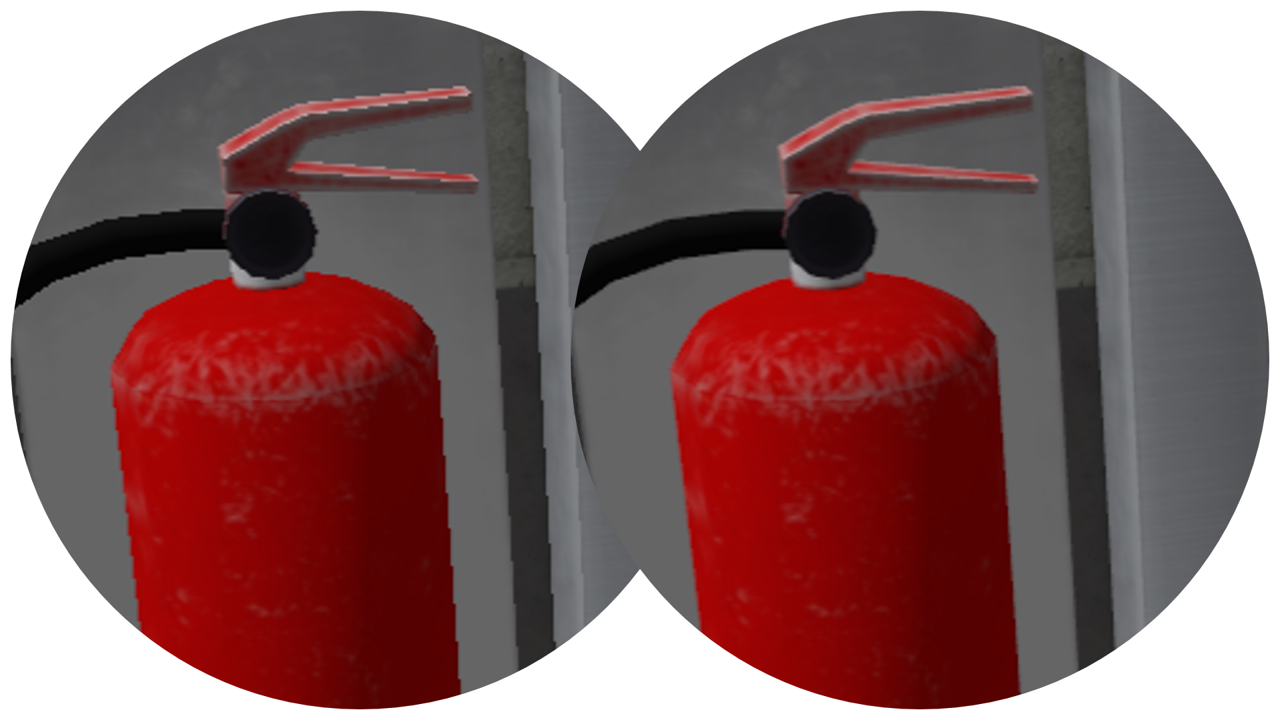
\includegraphics[width=1.0\textwidth]{figures/example_comparison_aliasing.png}
    \caption{Comparación de dos modelos, uno sin antialising y otro con antialiasing.}
    \label{fig:comparison-aliasing}
\end{figure}

En la figura \ref{fig:triangle-no-msaa} puede observarse cómo se evalúan los píxeles de un simple triángulo, quedando unos ``escalones'' muy prominentes. En la figura \ref{fig:triangle-msaa} se utiliza \textit{antialiasing MSAA}, en la que se suavizan los bordes alterando el color ligeramente.

\begin{figure}[htp]
    \centering
    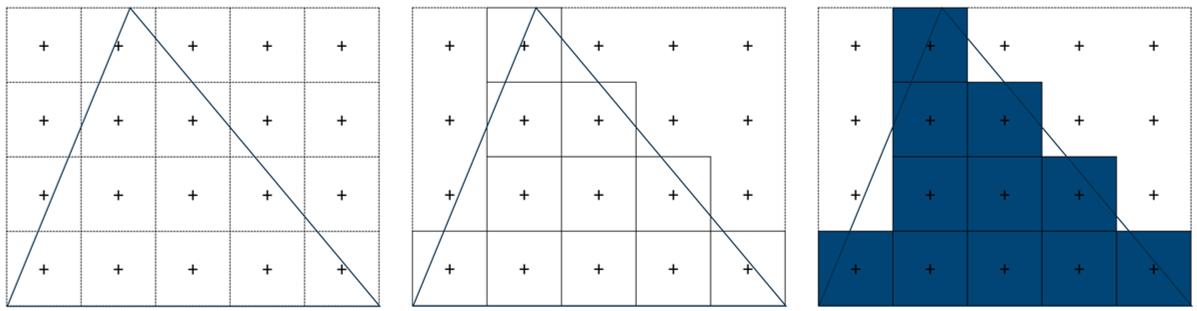
\includegraphics[width=1.0\textwidth]{figures/steps_no_msaa.png}
    \caption{Colores de un triángulo siendo evaluados sin antialiasing.}
    \label{fig:triangle-no-msaa}
\end{figure}

\begin{figure}[htp]
    \centering
    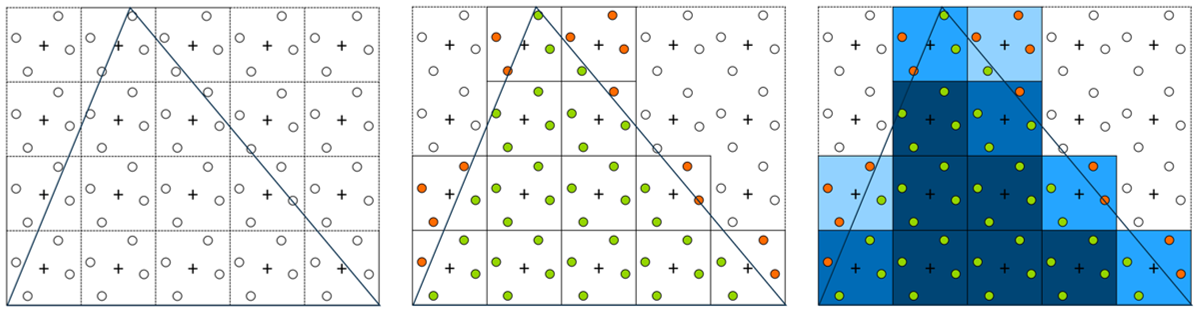
\includegraphics[width=1.0\textwidth]{figures/steps_msaa.png}
    \caption{Colores de un triángulo siendo evaluados con antialiasing MSAA}
    \label{fig:triangle-msaa}
\end{figure}

\section{APIs de Renderización} \label{sec:apis-render}

Entre las APIs de renderizado, destacan \textit{OpenGL} \cite{webKhronosOpenGL} y \textit{Vulkan} \cite{webKhronosOpenGL}, ambas desarrolladas por \textit{Khronos} \cite{webKhronos}. De hecho, \textit{OpenGL} es la predecesora de \textit{Vulkan} y se mantiene como una opción estable y sencilla de utilizar. 
Aunque \textit{Vulkan} es mucho más flexible, introduce complejidad; concretamente, está dirigido a aplicaciones muy demandantes que necesitan maximizar la eficiencia \cite{webNvidiaOglVulkan}.

\section{Implementaciones existentes} \label{sec:current-implementations}
Antes de abordar el desarrollo de un renderizador, ha sido necesario documentar sobre el funcionamiento de otros motores existentes, de forma que, aunque el propósito sea diferente, el análisis se ha centrado en las partes relacionadas con el proyecto. Cabe destacar que algunos motores, como \textit{Unity} o \textit{Unreal Engine}, son de software privativo y no pueden diseccionarse al detalle como podría hacerse con \textit{Godot}; en este caso, la única documentación disponible es el manual de usuario.

\subsection{Godot}

Renderización 2D \cite{webGodot2DRendererDocs} y 3D \cite{webGodot3DRendererDocs} acompañado de un motor de física. Incluye \textit{tilemaps}, partículas y animaciones. Se centra en luces, sombras, movimiento de partículas y visualización de \textit{meshes}. Usa \textit{OpenGL}, \textit{DirectX} y \textit{Vulkan} como \textit{APIs} de gráficos. Usa optimización \textit{GPU}. 

\paragraph{Luces y sombras}
Al igual que el resto del motor, las mecánicas de iluminación consisten en \textbf{nodos} o \textbf{vértices} en un grafo. Por ejemplo, \textit{DirectionalLight2D} \cite{webGodotDL2D} es usado para modelar la luz del sol o de la luna, \textit{CanvasModulate} \cite{webGodotCM} para dar color a la luz y, el elemento más común, \textit{PointLight2D} \cite{webGodotPL2D}, que es un punto de luz que podría ser una antorcha, fuego, proyectiles o similar. Para modelar sombra, se puede usar \textit{LightOccluder2D} \cite{webGodotLO2D}, indicando al \textit{shader} qué parte de la escena debe contener sombras.

\paragraph{2D Meshes}
Aunque menos usadas que los modelos \textit{3D}, dado que las imágenes son usadas con más frecuencia, \textit{Godot} da completo soporte a los modelos bidimensionales. También, es posible visualizar modelos tridimensionales a través de algunas herramientas en una escena de dos dimensiones. Permite convertir imágenes \textit{Sprite2D} \cite{webGodotSprite2D} a modelos 2D \textit{MeshInstance2D} \cite{webGodotMI2D}, ajustando parámetros según la calidad y rapidez que se requiera; puede ser mejor renderizar un modelo a partir de una imagen que directamente visualizar la imagen, especialmente con imágenes grandes, dibujando sólo las partes opacas e ignorando el resto

\paragraph{Animación 2D}
Hay dos formas de crear animación en dos dimensiones: a través de \textit{AnimatedSprite2D} \cite{webGodotAS2D}, una manera sencilla que sólo involucra cambio de textura, y \textit{AnimationPlayer} \cite{webGodotAP}, una manera más compleja que permite realizar más acciones en la animación, como reproducir sonidos, activar y desactivar \textit{hitboxes} \cite{webValveHitbox}, y demás. Se suele usar una plantilla de imágenes llamada \textit{sprite sheet} que recopila la animación en una sóla imagen, en vez de crear imágenes individuales para cada estado.

\paragraph{Antialiasing 2D}
Ofrece ajustes sobre el \textit{antialising} generales. Para las líneas puede activarse sin necesidad de \textit{MSAA}. Si se quiere utilizar el efecto sobre cualquier otra geometría, es necesario activar \textit{MSAA 2D} \cite{webGodotMSAA2D} en los ajustes del proyecto.

\paragraph{Shaders} \label{par:shaders-godot}
\textit{Godot} permite el uso de \textit{shaders} personalizados, con un lenguaje semejante \cite{webGodotShadingLanguage} a \textit{GLSL}, el lenguaje de \textit{OpenGL}. Los \textit{shaders} deben estar vinculados a un \textit{Material} \cite{webGodotMaterial} y este a un \textit{objeto}. Para interactuar con el \textit{shader} desde el código, se usan \textit{uniform}, de forma semejante a \textit{GLSL}, excepto que las funciones son propias del motor, como es \textit{set\_shader\_parameter}, indicando simplemente el nombre y el valor a actualizar, y \textit{get\_shader\_parameter} que recupera el valor de una variable indicando el nombre. Ambas funciones se definen en la clase \textit{Material}.
    
\subsection{Blender}
Renderización 2D y 3D. Tiene tres renderizadores, aunque el más relevante es \textit{Cycles} \cite{webBlenderCyclesDocs}. Basado en físicas, con objetivo de ser fotorrealista. Permite renderización \textit{multi-core} con \textit{CPU} y optimización \textit{SIMD}, a la vez que permite renderización mediante \textit{GPU} y \textit{multi-GPU}. La documentación no es particularmente extensa, aunque el motor es poderoso y cuenta con numerosas características \cite{webBlenderCyclesFeatures}, como pueden ser la iluminación, las sombras, las texturas y la perspectiva de cámara.

\subsection{GTK y GSK}
Apuesta por un renderer 2D unificado para \textit{OpenGL} y \textit{Vulkan}, que son compilados de la misma fuente, aunque este cambio es reciente. Previamente, existía un renderer 2D \textit{OpenGL} que usaban shaders simples aunque más optimizado.

El nuevo renderizador unificado se centra en la mantenibilidad y correción a largo plazo a cambio de rendimiento. Este lujo es posible gracias a que los programas que hacen uso de este software no son excesivamente demandantes ni requieren una tasa de rendimiento grande, como podrían \textit{Godot}, \textit{Blender}, \textit{Unity} o \textit{Unreal Engine}. También soporta algunas capacidades interesantes, como \textit{antialising}, escalado fraccional y gradientes arbitrarios. 

\paragraph{GSK}

\textit{GTK} \cite{webGTKDocs} aisla los mecanismos de renderización en una dependencia: \textit{GSK} \cite{webGSKDocs}. Con esta abstracción, puede funcionar sin comunicarse directamente con la \textit{API} en cuestión; lo mismo ocurre con los sistemas de ventanas: son abstraídos en una dependencia. \textit{GSK} ofrece una \textit{API} basada en caminos \cite{webGSKPathAPI}, usada para renderizar formas complejas; aunque también se usan para otros cometidos, como trayectorias en animación. El renderizado en \textit{GSK} se basa en \textbf{nodos}: clases con diferentes propósitos, construyendo un grafo el cual procesará un tipo de \textit{renderer}, según la \textit{API} gráfica deseada.

\subsection{Unity}
Renderer 3D y 2D que usa \textit{DirectX}, \textit{Metal}, \textit{OpenGL} y \textit{Vulkan}. Utiliza optimización \textit{GPU} para procesar el renderizado.
Proporcionan una página web como manual \cite{webUnityManual}, aunque la fuente es software privativo y el código público no está disponible.

\subsection{Conclusiones}
Existen numerosos sistemas de renderización \textit{2D} y \textit{3D} con diferentes propósitos: videojuegos, cine, modelado, etc. Muchos de ellos son públicos y su funcionamiento puede estudiarse.

La tabla \ref{tbl:comparison-engine} compara los motores mencionados: su capacidad dimensional, las \textit{APIs} que soportan, el propósito que tienen y su licencia de uso.

\begin{table}[htp]
\centering

    % Esta primera línea define las columnas de la tabla. Los posibles tipos de columna son:
    % c: texto centrado
    % l: texto alineado a la izquierda
    % r: texto centrado a la derecha
    % p: columna de ancho fijo
    % Las columnas tienen ancho dinámico según la anchura máxima de los elementos que contengan.

    % Las columnas l/r/c no parten el texto en filas diferentes si éste es demasiado largo. Para ello, puede utilizar el tipo de columna de ancho fijo "p".
    
    % Las barras verticales | se usan para definir los bordes verticales de la tabla. Pruebe a eliminar algunas y observe qué ocurre.
    \begin{tabular}{ | p{2cm} | p{2cm} | p{3cm} | p{3cm} | p{2cm} | }
        
        % A continuación van las filas de la tabla. En cada fila, las columnas se separan con el carácter &
        % Para terminar una fila se usa \\
        % Para incluir un borde horizontal entre filas se usa \hline

        % Cabecera con textos en negrita:
        \hline
        \textbf{Motor} & \textbf{2D/3D} & \textbf{APIs} & \textbf{Objetivo} & \textbf{Licencia}\\
        \hline
        
        % Cuerpo de la tabla:
        Godot & Ambos & OpenGL, Vulkan y DirectX & Videojuegos: partículas, animaciones, luces y sombras  & MIT\\
        \hline
        Blender & Ambos & CUDA, OptiX, HIP, oneAPI y Metal  & Fotorrealismo, basado en físicas  & GPL\\
        \hline
        GTK & 2D & OpenGL y Vulkan & Interfaces de usuario & GPL\\
        \hline
        Unity & Ambos & OpenGL, Vulkan, DirectX y Metal & Videojuegos y animación  & Privativa\\
        \hline
        
    \end{tabular} 
    
    \caption{Comparación de motores de renderización}
    \label{tbl:comparison-engine} 
\end{table}

Este proyecto pretende aportar a la escena existente una base sobre la que puede construirse un motor \textit{2D}, detallando los pasos dados para que incluso un programador inexperto en programación gráfica pueda iniciarse.


    \chapter{Análisis del problema}\label{chp:analysis}

En este capítulo se tratarán los requisitos \ref{sec:requirements} se ajustan al proyecto necesarios para el correcto funcionamiento del mismo.

\section{Requisitos}\label{sec:requirements}
La tabla de requisitos \ref{table:requirements} describe 4 tipos: \textbf{información} \ref{sub:information-requirement}, \textbf{funcional} \ref{sub:functional-requirement}, \textbf{no funcional} \ref{sub:non-functional-requirement} y \textbf{hardware} \ref{sub:hardware-requirement}. Cada elemento consta de un identificador, un número y una descripción.
\begin{table}[htp]
\centering

    % Esta primera línea define las columnas de la tabla. Los posibles tipos de columna son:
    % c: texto centrado
    % l: texto alineado a la izquierda
    % r: texto centrado a la derecha
    % p: columna de ancho fijo
    % Las columnas tienen ancho dinámico según la anchura máxima de los elementos que contengan.

    % Las columnas l/r/c no parten el texto en filas diferentes si éste es demasiado largo. Para ello, puede utilizar el tipo de columna de ancho fijo "p".
    
    % Las barras verticales | se usan para definir los bordes verticales de la tabla. Pruebe a eliminar algunas y observe qué ocurre.
    \begin{tabular}{ | p{3cm} | p{3cm} | p{3cm}| p{3cm} | }
        
        % A continuación van las filas de la tabla. En cada fila, las columnas se separan con el carácter &
        % Para terminar una fila se usa \\
        % Para incluir un borde horizontal entre filas se usa \hline

        % Cabecera con textos en negrita:
        \hline
        \textbf{Información} & \textbf{Funcionales} & \textbf{No funcionales} & \textbf{Hardware}\\
        \hline
        
        % Cuerpo de la tabla:
        I.01 Código GLSL & F.01 Biblioteca de shaders & NF.01 Robustez y detección de errores & H.01 Poseer una GPU configurada correctamente \\
        \hline
        I.02 Resultados, análisis y gráficas & F.02 Biblioteca de errores & NF.02 Modular y organizado & H.02 Sin mínima exigencia de CPU, RAM, disco, etc \\
        \hline
         & F.03 Biblioteca de polígonos & NF.03 Código comentado y en inglés & \\
        \hline
         & F.04 Biblioteca miscelánea de C & & \\
        \hline
         & F.05 Biblioteca de animación & & \\
        \hline
         & F.06 Ejemplo de uso y pruebas & & \\
        \hline
        
    \end{tabular} 
    
    \caption{Tabla de requisitos}
    \label{table:requirements} 
\end{table}


\subsection{Requisitos de información}\label{sub:information-requirement}
Los requisitos de información describen los documentos y código que debe ser almacenado, leído y procesado.

\begin{enumerate}

    \item \textit{Shaders}, código \textit{GLSL} externo que necesita ser compilado dentro del programa para renderizar la geometría.

    \item Resultados de los programas, almacenados en diferentes formatos con el objeto de llevar a cabo análisis de resultados y transformarlos en gráficas.
    
\end{enumerate}

\subsection{Requisitos funcionales}\label{sub:functional-requirement}
Los requisitos funcionales describen cómo se debe comportar el sistema al ser ejecutado y qué propiedades tiene.

\begin{enumerate}

    \item Debe existir una biblioteca relacionada con \textit{shaders} que facilite su uso para el usuario.

    \item Debe existir una biblioteca de errores que provea al usuario de una manera sencilla de comprobar la validez de ciertas acciones y actuar en consecuencia.

    \item Debe existir una biblioteca relacionada con \textbf{polígonos}, que construya geometría para el usuario.

    \item Debe existir una biblioteca miscelánea que cubra propósitos generales de programación, como leer archivos y crear estructuras de memoria.

    \item Debe existir una biblioteca de animación, que soporte crear una secuencia de transformaciones sobre los vértices en pantalla y que simulen movimiento, pudiendo configurar los fotogramas por segundo, acciones y demás.

    \item Deben existir programas que utilicen todas las bibliotecas creadas, para servir de ejemplo y sujeto de pruebas para los resultados a analizar.

\end{enumerate}

\subsection{Requisitos no funcionales}\label{sub:non-functional-requirement}
Los requisitos no funcionales describen características más abstractas a las funcionables que describen propiedades ajenas al comportamiento técnico del sistema, como pueden ser la robustez, la modularidad o la fluidez.

\begin{enumerate}

    \item El sistema debe ser robusto y detectar errores tras operaciones cruciales en la secuencia de los programas.
    
    \item El proyecto debe estar organizado de forma ordenada y modular.

    \item El código del proyecto debe estar comentado correctamente, además de estar escrito en el idioma inglés.
    
\end{enumerate}

\subsection{Requisitos hardware} \label{sub:hardware-requirement}

\begin{enumerate}
    \item Poseer una \textit{GPU}, preferiblemente \textit{AMD} o \textit{NVIDIA}, configurada correctamente con los controladores apropiados.

    \item No es necesario establecer un requisito mínimo de otros componentes, ya sea \textit{RAM}, \textit{CPU} o disco, pues \textit{OpenGL} es flexible.
\end{enumerate}


    \FloatBarrier
\chapter{Lenguaje y Tecnologías Empleadas} \label{chp:technologies}

Este capitulo aborda conceptos esenciales sobre las tecnologías usadas en el proyecto: lenguajes de programación, \textit{APIs} y herramientas de soporte. Concretamente, se trata el lenguaje \textit{C} \ref{sec:c-language}, utilizado durante todo el proyecto, las tecnologías de renderizado \ref{sec:render-technologies} y las herramientas de soporte utilizadas \ref{sec:support-technologies}.

\section{Lenguaje C} \label{sec:c-language}

\paragraph{Puntero}
Un \textbf{Puntero} es una variable que almacena una dirección en memoria de otra variable. 

Cabe mencionar que también es posible crear un puntero a una \textbf{función}:
\lstinputlisting[
    float,
    floatplacement=htp,
    language=C,
    label=cod:example-function-pointer,
    caption=Ejemplo de puntero a función en C
]{code/c_example_function_pointer.c}


\paragraph{Reserva y liberación de memoria}
En el lenguaje \textit{C}, la gestión de memoria \cite{webCppreferenceMemory} puede ser controlada por el usuario, lo que exige una gran responsabilidad por su parte. Aunque se prefiere siempre que sea posible que el sistema sea el que realice esta gestión, a veces es necesario: por ejemplo, una función que debe asignar espacio a un \textit{array} con un número de elementos no predefinido. En estos casos, puede hacerse uso de funciones como \textit{malloc} o \textit{calloc}, que inicializan memoria a petición del usuario; si se desea modificar el tamaño de esta memoria, puede utilizarse \textit{realloc} en lugar de una asignación nueva. Una vez terminadas las tareas pertinentes a la asignación de esta memoria solicitada, es necesario liberarla con \textit{free} y, para ser riguroso, darle un valor \textit{NULL} al puntero para evitar posibles confusiones respecto a la disponibilidad del mismo. 

\section{Tecnologías de renderizado} \label{sec:render-technologies}
En esta sección se describen, desde el punto de vista de la programación, las \textit{APIs} utilizadas.

Respecto a la sección \ref{sub:opengl}, que explica los conceptos pertenecientes a \textit{OpenGL} más importantes:
\begin{enumerate}

    \item En el apartado \ref{par:ogl-introduction} se presentan los conceptos necesarios de OpenGL. 
    
    \item En \ref{par:ogl-buffers} se describe cómo utilizar los \textit{buffers} con el fin de comunicarse con la \textit{GPU}.

    \item En \ref{par:ogl-shader-flow} se describe el flujo de \textit{shaders} que recorre una aplicación general que use \textit{OpenGl}.

    \item En \ref{par:ogl-uniforms} se explica el tipo de variable \textit{uniform}, utilizado para comunicarse directamente con valores de \textit{shaders}.

    \item En \ref{par:ogl-vertices-attributes} se describe cómo indicar al \textit{shader} qué valores utilizar y dónde se encuentran dentro de los \textit{buffers}, mencionados previamente.

    \item En \ref{par:ogl-shader-compilation} y \ref{par:ogl-program-creation} se describe con ejemplos de código el proceso para crear \textit{shaders} y un programa a partir de éstos.

    \item En la sección \ref{sub:glsl} se describe el lenguaje \textit{GLSL}, utilizado con el fin de programar \textit{shaders} para \textit{OpenGL}.
    
\end{enumerate}



\subsection{OpenGL} \label{sub:opengl}

Aunque también mencionado en el apartado \ref{sec:apis-render}, de las API existentes, \textit{OpenGL} y \textit{Vulkan}, en este trabajo se ha decidido usar \textit{OpenGL}, ya que es una \textit{API} muy utilizada y estable, a la par que altamente flexible (aunque no al nivel de \textit{Vulkan}).

\paragraph{Funcionamiento principal} \label{par:ogl-introduction}

Existen dos formas de utilizar \textit{OpenGl}: \textit{Immediate mode} y \textit{core-profile}. El primer modo es más fácil de entender y usar, aunque tiene funciones obsoletas y no se aconseja su uso. La manera recomendada de programar es con \textit{core-profile}, una división de la especificación con funcionalidades modernas. La especificación de \textit{OpenGL} permite extensiones para que los desarrolladores no necesiten esperar a una nueva versión.

\textit{OpenGL} se puede entender como una gran máquina de estados, llamándose a cada uno de ellos un \textbf{contexto}. Este contexto puede ser modificado por funciones y utilizado por otras. El código está escrito en \textit{C}, aunque permite derivaciones para distintos lenguajes. Se usan \textbf{objetos}: cada objeto es un conjunto de opciones que representan un \textit{subset} del estado de \textit{OpenGL}. Por ejemplo, un objeto podría representar el tamaño y colores de una ventana.

Los objetos se crean, se modifican y se utilizan mediante la \textit{API}, y la información se almacena fuera de la vista del programador. Esto permite una flexibilidad y reusabilidad increíble, pues se pueden crear varios objetos y vincularlos para dibujarlos de forma rápida.

El extracto de código \ref{cod:example-opengl-object} podría ser (son comandos ficticios) un ejemplo de creación y manipulación de un objeto:
\lstinputlisting[
    float,
    floatplacement=!htp,
    language=C,
    label=cod:example-opengl-object,
    caption=Ejemplo de objeto en OpenGL
]{code/c_example_opengl_object.c}

\paragraph{Buffers} \label{par:ogl-buffers}

A continuación se detallará la especificación de vértices \cite{webVertexSpecDocs} en \textit{OpenGL}.

\begin{itemize}
    \item El \textit{Vertex Buffer Object} (VBO) es un\textit{buffer} que puede almacenar una gran cantidad de vértices en memoria. El objetivo es envíar el mayor número de datos a la vez posible.

    \item Un \textit{Vertex Array Object} (VAO) es un \textit{buffer} enlazable, como es el \textit{VBO}. Almacena la configuración de los atributos de los vértices. Está fuertemente vinculado al \textit{VBO}, ya que el \textit{VAO} almacena la configuración de los vértices almacenados en él. El \textit{VAO} almacena las llamadas a atributos y vértices, por lo que para dibujar, una vez configurado, sería necesario simplemente vincularlo. Cabe mencionar que, si la configuración o el \textit{VBO} cambiase, sería necesario actualizar el \textit{VAO}.

    \item Un \textit{Element Buffer Object} (EBO), también llamado \textit{Index Buffer}, permite almacenar en él indices que referencian vértices en el \textit{VBO}. En vez de duplicar vértices, pueden referenciarse múltiples veces. Por ejemplo, un cuadrado contiene 2 triángulos y 6 vértices. Utilizando un \textit{EBO}, podrían declararse 4 vértices e indicar el orden en el que se utilizan para crear los triángulos.
\end{itemize}

En el ejemplo \ref{cod:example-creation-vbo-vao} se muestra un ejemplo de creación de los \textit{buffers VBO} y \textit{VAO}. Una vez creados y configurados, en la función \textit{display} ha de vincularse el \textit{VAO} para cargar los vértices y su configuración, como en el ejemplo \ref{cod:example-usage-vbo-vao}.
\lstinputlisting[
    float,
    floatplacement=!htp,
    language=C,
    label=cod:example-creation-vbo-vao,
    caption=Ejemplo de creación de los objetos VBO y VAO.
]{code/c_example_creation_vbo_vao.c}

\lstinputlisting[
    float,
    floatplacement=!htp,
    language=C,
    label=cod:example-usage-vbo-vao,
    caption=Ejemplo de uso de los objetos VBO y VAO.
]{code/c_example_usage_vbo_vao.c}

\FloatBarrier

El \textit{EBO} puede usarse para dibujar un cuadrado. Se debe añadir después de vincular el \textit{VAO}, dejando el resto de la misma manera. La función de \textit{display} es idéntica, aunque se sustituye \textit{glDrawArrays} por \textit{glDrawElements}. El ejemplo \ref{cod:example-creation-ebo} se muestra la creación de este \textit{buffer EBO} y en el ejemplo \ref{cod:example-usage-ebo} el uso de éste.

\lstinputlisting[
    float,
    floatplacement=!htp,
    language=C,
    label=cod:example-creation-ebo,
    caption=Ejemplo de creación de EBO.
]{code/c_example_creation_ebo.c}

\lstinputlisting[
    float,
    floatplacement=!htp,
    language=C,
    label=cod:example-usage-ebo,
    caption=Ejemplo de uso de EBO.
]{code/c_example_usage_ebo.c}

\FloatBarrier
\paragraph{Flujo de shaders} \label{par:ogl-shader-flow}

El flujo de shaders \cite{webOGLShaderPipe} de \textit{OpenGL} puede dividirse en 6 etapas fundamentales: \textit{Vertex Shader}, \textit{Tesselation}, \textit{Geometry Shader}, \textit{Primitive Assembly}, \textit{Rasterization}, \textit{Fragment Shader} y \textit{Tests and Blending}. Hay algunas fases en las que el programador puede introducir su propia implementación, como se mostrará más adelante.

Se usa un lenguaje especial de \textit{OpenGL} para \textit{shaders}, llamado \textit{GLSL}, para compilar y generar estos \textit{shaders}. Este lenguaje se tratará más adelante.

\begin{enumerate}
    \item \textbf{Vertex Shader}. Se transforman vectores de posición de los vértices en otros diferentes, generalmente 3D.
    
    \item \textbf{Tessellation}. Se subdivide la geometría compleja en Primitivos más simples.
    
    \item \textbf{Geometry Shader}. Se modifican, añaden o eliminan formas. Por ejemplo, romper un triángulo en tres, eliminar formas que no necesita o cambiar un punto en un cuadrado.
    
    \item \textbf{Primitive Assembly}. Se toman los vértices procesados y se agrupan en formas simples, como puntos, líneas o triángulos.
    
    \item \textbf{Rasterization}. Se transforman formas 3D en piezas 2D llamadas fragmentos (potenciales píxeles). En esta fase se determina qué píxeles en la pantalla cubre cada forma y qué datos lleva cada fragmento.
    
    \item \textbf{Fragment Shader}. En este paso se decide cómo se verá cada fragmento, es decir, color, luces, sombras, textura, etc.
    
    \item \textbf{Tests and Blending} (Per-Sample Operations). En este paso final se decide qué fragmentos finalmente ocuparán píxeles en la pantalla. Se hacen pruebas como el \textit{Depth Test}, el \textit{Stencil Test} o el \textit{Scissor Test}. Después de estas pruebas se crea la imagen final con los fragmentos restantes.

\end{enumerate}

\begin{figure}[htp]
    \centering
    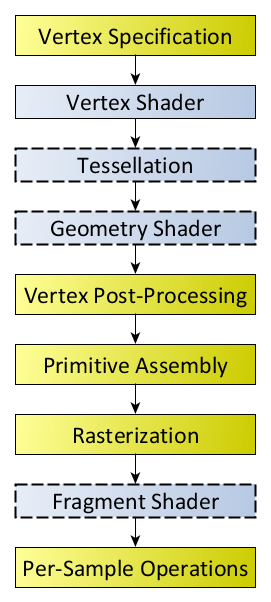
\includegraphics[height=0.8\textheight]{figures/diagrams/RenderingPipeline.png}
    \caption{Diagrama de Khronos que describe el flujo de shaders en OpenGL.}
    \label{fig:shader-pipeline}
\end{figure}

\FloatBarrier
\paragraph{Uniforms} \label{par:ogl-uniforms}

Los \textit{uniforms} son una manera de enviar datos de la aplicación en \textit{CPU} a los \textit{shaders} en \textit{GPU}. Son variables globales y pueden ser accedidas por cualquier \textit{shader}. Se añade la palabra clave \textit{uniform} a la variable en el \textit{shader} para convertirla en \textit{uniform}. Esta variable debe ser declarada en el \textit{shader}, de la misma forma que cualquier variable en \textit{GLSL}, aunque con el prefijo \textit{uniform}. Para acceder a ella desde el código \textit{C}, primero se debe localizar el atributo y entonces, dar un valor a la variable. En la figura \ref{cod:example-uniform} se muestra un ejemplo.

\lstinputlisting[
    float,
    floatplacement=!htp,
    language=C,
    label=cod:example-uniform,
    caption=Ejemplo de uso de variables Uniform.
]{code/c_example_uniform.c}

\FloatBarrier
\paragraph{Atributos de vértices} \label{par:ogl-vertices-attributes}

Para indicarle a \textit{OpenGL} cómo utilizar los datos que ha recibido, es necesario indicarlo explícitamente. Por ejemplo, si los vértices tienen 3 coordenadas, siendo cada una de ellas float, que usualmente son 4 bytes, esto significa que cada vértice serán 12 bytes, y si el polígono deseado fuera un triángulo, serían 3 vértices: 36 bytes. Se debe tener en cuenta que no hay espacio entre los valores en este caso. Un ejemplo de configuración de atributos sería la figura \ref{cod:example-attributes}.

\lstinputlisting[
    float,
    floatplacement=!htp,
    language=C,
    label=cod:example-attributes,
    caption=Ejemplo de configuración de atributos.
]{code/c_example_attributes.c}

Los argumentos de \textit{glVertexAttribPointer} son:
\begin{enumerate}
    \item \textbf{Índice}. Posición del atributo. Puede definirse en el shader o conseguirse dinámicamente.

    \item \textbf{Tamaño} del atributo. 

    \item \textbf{Tipo} de dato. Las coordenadas se guardan como \textit{float}.

    \item \textbf{Normalización}. En este caso, las coordenadas están ya normalizadas previamente, por lo que se deja en falso.

    \item \textbf{Stride}. Es el espacio entre atributos consecutivos. Si es \textit{0}, se asumirá que los datos siguen uno detrás del otro sin espacio entre ellos.

    \item \textbf{Offset}. Es donde empieza la posición de los datos en el \textit{buffer}. Requiere un puntero a \textit{void}.

\end{enumerate}

\FloatBarrier
\paragraph{Compilación de un shader} \label{par:ogl-shader-compilation}

Con el propósito de mantener la sencillez en el ejemplo, el código \textit{GLSL} se almacenará en constantes dentro del código \textit{C}, el cual se le proporciona a \textit{OpenGL} y se compila; en el ejemplo \ref{cod:example-shader-compilation} se muestra este concepto.

\lstinputlisting[
    float,
    floatplacement=!htp,
    language=C,
    label=cod:example-shader-compilation,
    caption=Ejemplo de compilación de un shader
]{code/c_example_shader_compilation.c}

\FloatBarrier
\paragraph{Creación de un programa} \label{par:ogl-program-creation}

Una vez se tienen los \textit{shaders} compilados por separado, es necesario enlazarlos para combinarlos. Esto se hace mediante un \textbf{programa}. Se vinculan los shaders a este programa, que se activa cuando se renderizan objetos. Las salidas de cada \textit{shader}, entonces, se vinculan a las entradas del siguiente. El código necesario para la creación del programa podría ser como el de la figura \ref{cod:example-shader-program}.

\lstinputlisting[
    float,
    floatplacement=!htp,
    language=C,
    label=cod:example-shader-program,
    caption=Ejemplo de creación de un programa
]{code/c_example_shader_program.c}

\subsection{GLSL} \label{sub:glsl}

Los shaders deben ser compilados en tiempo de ejecución. Aunque no  se haya profundizado en el lenguaje \textit{GLSL} \cite{webGLSLDocs}, es sencillo de entender una vez aprendido \textit{C}.

El código de la figura \ref{cod:example-vertex-shader} es un ejemplo muy básico de un \textit{Vertex Shader} que simplemente pasa las coordenadas al \textit{shader}, sin manipularlas:
\lstinputlisting[
    float,
    floatplacement=!htp,
    language=GLSL,
    label=cod:example-vertex-shader,
    caption=Ejemplo de Vertex Shader
]{code/glsl_example_vertex_shader.vert}

La primera línea indica la versión que se utiliza, que es semejante a la versión de \textit{OpenGL} que se esté usando (3.3). La segunda línea indica la posición en la que se encuentra el dato \textit{aPos}, que es un vector de 3 dimensiones. Este sería el vector que indica la posición de un vértice. La posición se transporta a un vector de 4 dimensiones, en la que la última coordenada es un dato llamado \textit{perspective division}, en la función principal del \textit{shader}.

\FloatBarrier

El código de la figura \ref{cod:example-fragment-shader} es un ejemplo muy básico de un \textit{Fragment Shader} que hace que todos los colores sean el naranja.

\lstinputlisting[
    float,
    floatplacement=!htp,
    language=GLSL,
    label=cod:example-fragment-shader,
    caption=Ejemplo de Fragment Shader
]{code/glsl_example_fragment_shader.frag}

La instrucción out hace que devuelva una variable: \textit{FragColor}, que decide el color final. En este caso, es un vector de 4 dimensiones, que indica los tres colores primarios: rojo, verde y azul (RGB) y el valor alpha (opacidad).

\FloatBarrier
\section{Herramientas de soporte} \label{sec:support-technologies}

En esta sección se tratarán herramientas de soporte, útiles para la gestión y organización del proyecto, tanto en la estructura como en el código, tales como \textit{CMake} \ref{sub:support-cmake}, que gestiona la compilación y dependencias, \textit{GLEW} \ref{sub:support-glew}, que elimina la necesidad de obtener las funciones de \textit{OpenGL} manualmente, \textit{Freeglut} \ref{sub:support-freeglut}, que gestiona la creación de ventanas, o \textit{Git} \ref{sub:support-git}, que gestiona el control de versiones.

\subsection{CMake} \label{sub:support-cmake}
Se usará \textit{CMake} \cite{webCMakeDocs} para gestionar dependencias y compilación del proyecto.

\textit{CMake} maneja dependencias de forma estable y es beneficioso a largo plazo, cuando el código empieza a aumentar de tamaño y comienza a ser insostenible compilar a mano. Otra alternativa sería manualmente escribir \textit{Makefile}. Se consideró más útil y profesional usar \textit{CMake}, ya que tiene un nivel de abstracción sobre los \textit{Makefile} muy pulido y efectivo que costaría replicar a mano.

\FloatBarrier
\subsection{GLEW} \label{sub:support-glew}
Las funciones de \textit{OpenGL} se cargan de maneras diferentes según la plataforma en la que nos encontremos. En \textit{GNU/Linux}, bajo la implementación de \textit{Mesa} \cite{webMesaDocs}, están dinámicamente enlazadas, por lo que hay que recuperarlas de memoria. En otras plataformas es distinto, por lo que \textit{GLEW} es muy útil para resolver este problema.

\textit{GLEW} \cite{webGLEW} inicializa las funciones de \textit{OpenGL} de forma agnóstica al sistema operativo. Esto libera al programador de una tediosa carga, pues hacerlo de forma manual sería fatigador y la mejora en rendimiento sería mínima o nula. El código necesario para la inicialización de \textit{GLEW} es sencillo y se muestra en la figura \ref{cod:example-glew}.

\lstinputlisting[
    float,
    floatplacement=!htp,
    language=C,
    label=cod:example-glew,
    caption=Ejemplo de inicialización de GLEW
]{code/c_example_glew.c}

\FloatBarrier
\subsection{Freeglut} \label{sub:support-freeglut}
\textit{Freeglut} \cite{webFreeglut} nace como alternativa a \textit{GLUT} \cite{specsGLUT}, una biblioteca ya abandonada. Se encarga de todas las tareas específicas al sistema operativo necesarias para crear ventanas, inicializar contextos de \textit{OpenGL}, gestionar eventos de entrada y permite crear programas realmente portables con \textit{OpenGL}. El codigo necesario para inicializar \textit{Freeglut} podría ser como en la figura \ref{cod:example-glut}:

\lstinputlisting[
    float,
    floatplacement=!htp,
    language=C,
    label=cod:example-glut,
    caption=Ejemplo de inicialización de Freeglut
]{code/c_example_glut.c}

\FloatBarrier

\subsection{Git} \label{sub:support-git}

La tecnología \textit{Git} se ha utilizado durante todo el proyecto como software de \textbf{control de versiones}, haciendo gran uso de las ramas para distintas funcionalidades, las cuales evitan un posible colapso irremediable permitiendo deshacer cambios rápidamente.

    \chapter{Diseño del sistema} \label{chp:design}

En este capítulo se detalla el diseño del sistema, especificando a alto nivel cada parte que lo compone, incluyendo, también, esquemas que ilustran su estructura. Concretamente, se describirán las bibliotecas de \textit{\textbf{shaders}} \ref{sec:lib-shaders}, \textbf{errores} \ref{sec:lib-errors}, código \textbf{misceláneo } \textit{C} \ref{sec:lib-misc-c}, \textbf{polígonos} \ref{sec:lib-polygon} y \textbf{animaciones} \ref{sec:lib-animation}. En cada una de estas secciones, se tratan las decisiones de diseño tomadas respecto a cada biblioteca donde se expone cada elemento de la biblioteca y unas directrices sobre cómo utilizarlas desde la perspectiva del usuario.

\section{Leyenda}

La figura \ref{fig:lib-legend} es la leyenda que representa los elementos con los que se describe el sistema en los próximos diagramas de bibliotecas.

A continuación, se describen los diferentes componentes de sistema acompañados de diagramas que indican los elementos que lo componen y su relación:
\begin{itemize}
    \item \textbf{Lista azul}: indica una estructura de datos.
    \item \textbf{Lista verde}: indica un tipo \textbf{enumerado}.
    \item \textbf{Rectángulo}: indica una función o \textit{macro} 
    \item \textbf{Flechas}: indican la dependencia entre elementos, de forma que el elemento origen es la dependencia del elemento destino.
\end{itemize}

En los sucesivos apartados, se describen cada uno de los módulos que componen el sistema, comenzando por la biblioteca de \textit{shaders}. La figura \ref{fig:libraries-overview} muestra la estructura general de las bibliotecas empleadas en el proyecto y las relaciones de dependencia entre ellas.

\begin{figure}[htp]
    \centering
    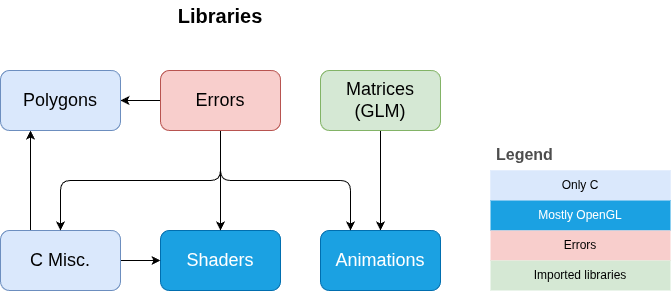
\includegraphics[width=0.9\textwidth]{figures/diagrams/libraries.png}
    \caption{Diagrama general de las bibliotecas y sus relaciones.}
    \label{fig:libraries-overview}
\end{figure}

\begin{figure}[htp]
    \centering
    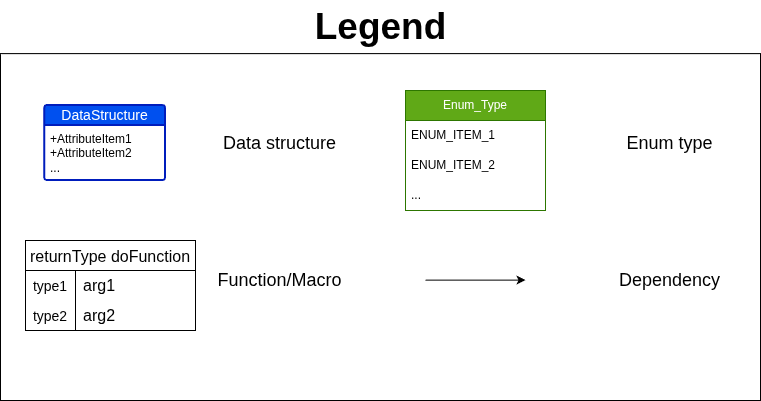
\includegraphics[width=0.7\textwidth]{figures/diagrams/libraries_legend.png}
    \caption{Leyenda de los diagramas de las bibliotecas.}
    \label{fig:lib-legend}
\end{figure}

\section{Shaders} \label{sec:lib-shaders}

En esta sección se trata la biblioteca de \textit{shaders}: su motivación, funciones, estructuras de datos y la \textit{API} pública que ofrece. En la figura \ref{fig:graph-libraries-shader} se representa la estructura de la biblioteca de \textit{shaders}, la cual existe con el propósito de facilitar el procesamiento de los mismos, en lugar de manualmente repetir el proceso cada vez que se deseen usar. Así, no es necesario leer, compilar y enlazar los \textit{shaders} manualmente.

\begin{figure}[htp]
    \centering
    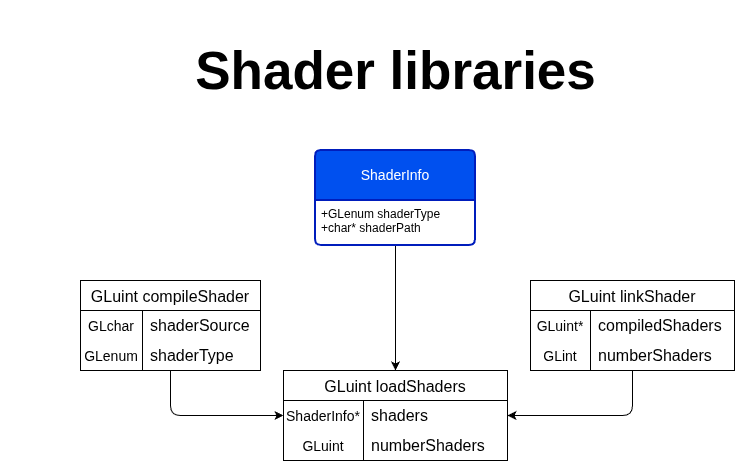
\includegraphics[width=0.9\textwidth]{figures/diagrams/libraries_shader.png}
    \caption{Diagrama de la biblioteca de shaders.}
    \label{fig:graph-libraries-shader}
\end{figure}

\subsection{Decisiones de diseño}

\lstinputlisting[
    float,
    floatplacement=!htp,
    language=C,
    label=cod:headers-shader-libraries,
    caption=Prototipos de la biblioteca de shaders
]{code/h_shader_libraries.h}

El código \ref{cod:headers-shader-libraries} muestra el prototipo de la biblioteca en código \textit{C}.

\begin{itemize}

    \item La estructura \textit{ShaderInfo} contiene el tipo del \textit{shader} y una cadena de caracteres contenido la ruta hacia el shader.
    
    \item Se ha separado el proceso del \textit{shader} en dos funciones que los compilan y enlazan en un programa: \textit{compileShader} y \textit{linkShader}. Luego, se utilizan las dos juntas en la función \textit{loadShader} junto a los datos recibidos en la estructura \textit{ShaderInfo}. De esta manera, en lugar de una sóla función con muchos argumentos que realice muchas tareas, se divide en varias partes y cooperan entre ellas.
    \begin{enumerate}
        \item La función \textit{compileShader} toma el contenido y el tipo del \textit{shader} para luego compilarlo. Devuelve su identificador como número entero sin signo.

        \item La función \textit{linkShader} toma una lista de \textit{shaders} compilados, es decir, sus identificadores, y los enlaza creando un programa. Devuelve su identificador como número entero sin signo.

        \item La función \textit{loadShaders} toma una lista de \textit{ShaderInfo} y los procesa utilizando las dos funciones anteriores, generando un programa. Para cada \textit{shader}, lee su contenido del fichero en la ruta correspondiente y lo compila según el tipo; los dos datos proporcionados por \textit{ShaderInfo}. Una vez compilados todos, se enlazan en un sólo programa. Devuelve su identificador como número entero sin signo.
        
    \end{enumerate}
    
\end{itemize}

\subsection{API pública}
El usuario deberá utilizar \textit{ShaderInfo}, completándola con los datos del tipo del \textit{shader} y su contenido en forma de cadena de caracteres. Posteriormente, llamar a la función \textit{loadShader} recibiendo estos datos; aunque se deja libertad para realizar el proceso manualmente, pudiendo llamar por separado a \textit{compileShader} y \textit{linkShader}.

\begin{itemize}
    \item Funciones internas:
    \begin{itemize}
        \item \textit{compileShader}.
        \item \textit{linkShader}.
    \end{itemize}
    
    \item Funciones públicas:
    \begin{itemize}
        \item \textit{loadShader}.
    \end{itemize}
    
    \item Estructuras públicas:
    \begin{itemize}
        \item \textit{ShaderInfo}.
    \end{itemize}
\end{itemize}

\section{Errores} \label{sec:lib-errors}

En esta sección se trata la biblioteca de \textbf{errores}: su motivación, funciones, estructuras de datos y la \textit{API} pública que ofrece. La figura \ref{fig:graph-libraries-error} representa la biblioteca de errores, que tiene como objetivo comprobar si el valor recibido es adecuado y proporcionar mensajes de error, a la vez que devuelve un número que indica si fue válido o no. De esta manera, se centralizan los errores y se reduce la comprobación caótica de ellos en el código. También, sería sencillo determinar qué tipo de error se intenta comprobar al revisar el código.

\begin{figure}[htp]
    \centering
    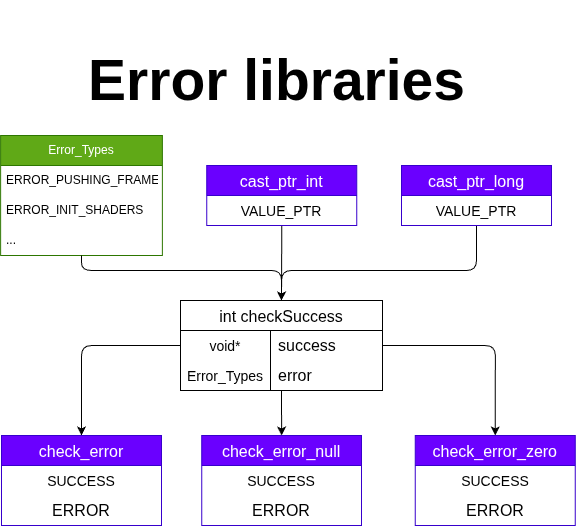
\includegraphics[width=0.9\textwidth]{figures/diagrams/libraries_error.png}
    \caption{Diagrama de la biblioteca de errores.}
    \label{fig:graph-libraries-error}
\end{figure}

\subsection{Decisiones de diseño}

\lstinputlisting[
    float,
    floatplacement=!htp,
    language=C,
    label=cod:headers-errors-libraries,
    caption=Prototipos de la biblioteca de errores
]{code/h_errors_libraries.h}

El código \ref{cod:headers-errors-libraries} muestra el prototipo de la biblioteca en código \textit{C}.

\begin{itemize}

    \item Se recopilan los tipos de errores en un enumerado llamado \textit{Error\_Types}: se organizan mediante texto y se traducen a números. De esta forma, es fácil distinguir qué error se pretende comprobar sin perder eficiencia.

    \item La función principal es \textit{checkSuccess}, que comprueba la validez de un valor según un tipo de error. Se utilizan también funciones \textit{macro} auxiliares para convertir tipos y retornar.
    \begin{enumerate}
    
        \item La función \textit{checkSuccess} toma una dirección a un valor y el tipo de error que se quiere comprobar, con el que se decide a qué tipo se debe transformar el valor y qué condición evaluar. De esta forma, puede determinarse qué tipo es el valor original sin crear demasiadas funciones. Por supuesto, conllevaría sus riesgos, concretamente en el mal uso del usuario al enviar los datos. Devuelve 0 en éxito y 1 en fracaso.

        \item Las funciones \textit{macro} \textit{cast\_ptr\_int} y \textit{cast\_ptr\_long} toman una dirección a un valor y devuelven ese mismo valor convertido al tipo \textit{int} o \textit{long}, respectivamente.

        \item En el caso de que se desee retornar un valor y finalizar la función en caso de que sea inválido, se han diseñado unas funciones \textit{macro} que comprueban la salida de \textit{checkSuccess} y devuelven un valor deseado: \textit{check\_error}, \textit{check\_error\_null}, \textit{check\_error\_zero}, que devuelven negativo, nulo y cero, respectivamente.
        
    \end{enumerate}

\end{itemize}

\subsection{API pública}
El usuario debería, tras una función crítica, comprobar el valor, ya sea llamando a alguna de las \textit{macros} o \textit{checkSuccess}, dependiendo de si se quiere devolver un valor o no.

\section{Misceláneo} \label{sec:lib-misc-c}

En esta sección se detalla la biblioteca de funciones \textbf{misceláneas}: su motivación, funciones, estructuras de datos y la \textit{API} pública que ofrece.

En la biblioteca miscelánea de \textit{C} \ref{fig:graph-libraries-miscc} se reúnen funciones auxiliares no dirigidas especialmente a \textit{OpenGL} y compuestas por código \textit{C} sin dependencias. Principalmente, se ha diseñado con la intención de ser utilizada para la lectura de ficheros, la creación de estructuras de datos y otras cuestiones generales de programación en \textit{C}.

\begin{figure}[htp]
    \centering
    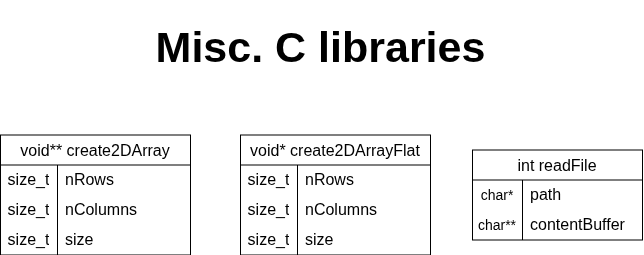
\includegraphics[width=1.0\textwidth]{figures/diagrams/libraries_miscc.png}
    \caption{Diagrama de la biblioteca de funciones misceláneas de C.}
    \label{fig:graph-libraries-miscc}
\end{figure}


\subsection{Decisiones de diseño}

\lstinputlisting[
    float,
    floatplacement=!htp,
    language=C,
    label=cod:headers-miscc-libraries,
    caption=Prototipos de la biblioteca miscelánea
]{code/h_miscc_libraries.h}

El código \ref{cod:headers-miscc-libraries} muestra el prototipo de la biblioteca en código \textit{C}.

\begin{itemize}
    \item Para leer archivos se crea la función \textit{readFile}. Se crean las funciones \textit{create2DArray} y \textit{create2DArrayFlat} para, rápidamente, asignar memoria a una estructura de datos en forma de lista de listas o una sóla lista aplanada. 
    \begin{enumerate}
        \item La función \textit{readFile} toma una ruta hacia un fichero y almacena sus contenidos en un \textit{buffer}. Se realiza la lectura de un fichero cada vez que se procesa un \textit{shader}, por lo que es una función muy conveniente.

        \item Se crean las funciones \textit{create2DArray} y \textit{create2DArrayFlat} para crear una matriz \textit{2D}. La primera función consistiría en crear una lista de listas, mientras que en la segunda está aplanada, es decir, los elementos son consecutivos. Principalmente, están pensadas para utilizarse en la creación de matrices de coordenadas bidimensionales.
    \end{enumerate}
    
\end{itemize}

\subsection{API pública}
El usuario debería utilizar \textit{readFile} aportando una ruta hacia un fichero y un \textit{buffer} donde asignar memoria y almacenar sus contenidos.

Las restantes dos funciones deberían utilizarse aportando el tamaño de las columnas y filas, además de un \textit{buffer}, semejante al de \textit{readFile}. Entonces, el \textit{buffer}, aunque vacío, tendrá asignada la memoria deseada para una matriz bidimensional.

\section{Polígonos} \label{sec:lib-polygon}
En esta sección se trata la biblioteca de \textbf{polígonos}: su motivación, funciones, estructuras de datos y la \textit{API} pública que ofrece.

\subsection{Decisiones de diseño}

Esta biblioteca de polígonos \ref{fig:graph-libraries-polygon} trata la creación de polígonos. En esta versión es bastante reducida y en futuras versiones se espera un crecimiento en las funcionalidades. La función principal crea un polígono regular de un número de vértices. En lugar de crear manualmente polígonos vértice a vértice, esta biblioteca sirve al usuario para generarlos automáticamente con algunos parámetros.

\begin{itemize}

    \item El programa \textit{createNGonVertices} construye un polígono regular de $n$ vértices en el centro de la pantalla, junto a un \textit{offset} para mover el polígono a otra coordenadas diferentes del origen. Estas coordenadas se almacenan consecutivamente como una matriz 2D plana, utilizando la función anteriormente descrita \textit{create2DArrayFlat}. Calcula los puntos a partir de las ecuaciones de las coordenadas polares \ref{equ:polar-coordinates}, siendo $t$ un ángulo interior que se calcula con la ecuación \ref{equ:internal-angle}. Divide el ángulo completo entre el número de vértices multiplicado por el índice del vértice y le suma un ángulo constante. De esta forma, se calcula cada ángulo perteneciente a cada vértice y sus coordenadas asociadas.
    
\end{itemize}

\begin{figure}[htp]
    \begin{equation}
        x = r * cos(t), y = r * sin(t)
    \end{equation}
    \caption{Ecuación de las coordenadas polares en dos dimensiones}
    \label{equ:polar-coordinates} 
\end{figure} 

\begin{figure}[htp]
    \begin{equation}
        t = \pi*i/n + \pi/2
    \end{equation}
    \caption{Ecuación del ángulo interno en un polígono}
    \label{equ:internal-angle} 
\end{figure} 

\lstinputlisting[
    float,
    floatplacement=!htp,
    language=C,
    label=cod:headers-polygon-libraries,
    caption=Prototipos de la biblioteca de polígonos
]{code/h_polygon_libraries.h}

El código \ref{cod:headers-polygon-libraries} muestra el prototipo de la biblioteca en código \textit{C}.

\begin{figure}[htp]
    \centering
    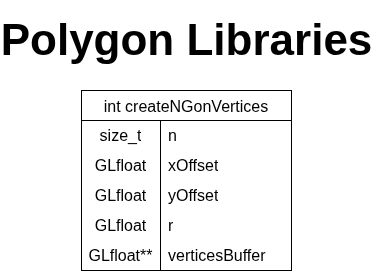
\includegraphics[width=0.7\textwidth]{figures/diagrams/libraries_polygon.png}
    \caption{Diagrama de la biblioteca de polígonos.}
    \label{fig:graph-libraries-polygon}
\end{figure}

\subsection{API pública}
El usuario debería utilizar la función \textit{createNGonVertices} para crear un polígono regular de $n$ vértices, aportando un \textit{buffer} donde almacenarlos y unas coordenadas bidimensionales que servirán de desplazamiento desde el centro de la pantalla.

Una vez calculados los vértices y sus coordenadas queda calcular la distribución de los triángulos dentro de este polígono. Pueden ser representados como un \textit{triangle fan} y exactamente $n-2$ triángulos; en OpenGL se asigna $GL\_TRIANGLE\_FAN$ en la función que dibuja el polígono. El primer vértice actúa de nodo principal y cada pareja de vértices posteriores se conecta al primero.

\section{Animaciones} \label{sec:lib-animation}

En esta sección se trata la biblioteca de \textbf{animaciones} \ref{fig:graph-libraries-animation} su motivación, funciones, estructuras de datos y la \textit{API} pública que ofrece.

Se ha creado esta biblioteca con el propósito de facilitar la animación de geometría, permitiendo mover, escalar y rotar, ya sea cargando de una vez una serie de transformaciones o una a una. Gestiona los fotogramas y la acción en cada uno de ellos, aunque con un alto grado de personalización.

\begin{figure}[htp]
    \begin{subfigure}[t]{1.0\textwidth}
        \centering
        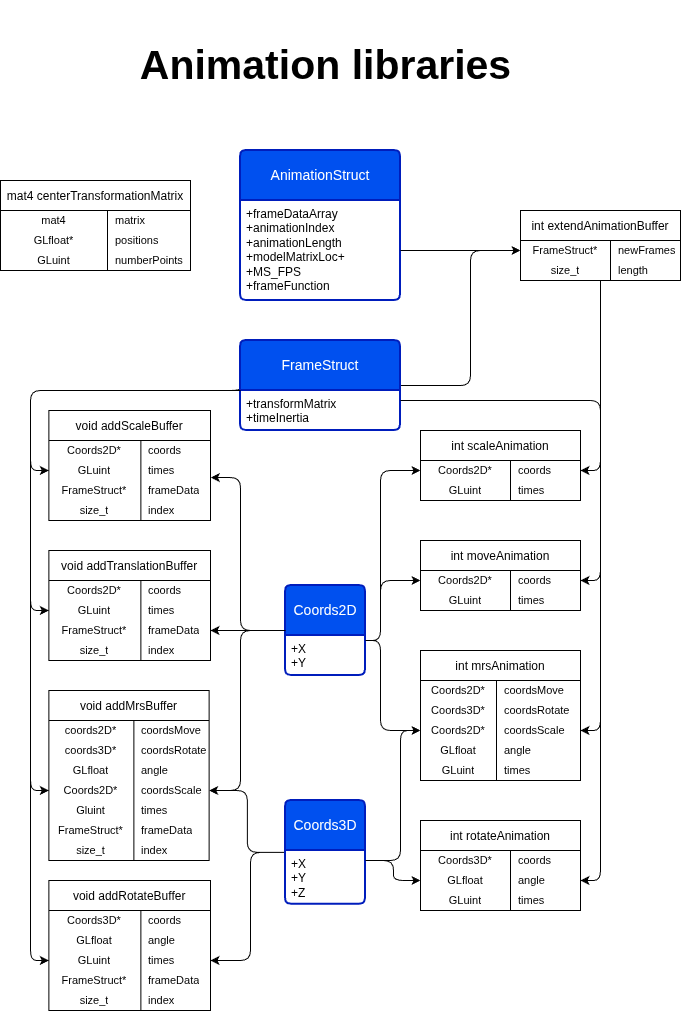
\includegraphics[width=1.0\textwidth]{figures/diagrams/libraries_animation1.png}
        \caption{Diagrama de la biblioteca de animaciones; parte 1.}
        \label{fig:graph-libraries-animation1}
    \end{subfigure}
\end{figure}
    
\begin{figure}[htp]
    \begin{subfigure}[t]{1.0\textwidth}
        \ContinuedFloat
        \centering
        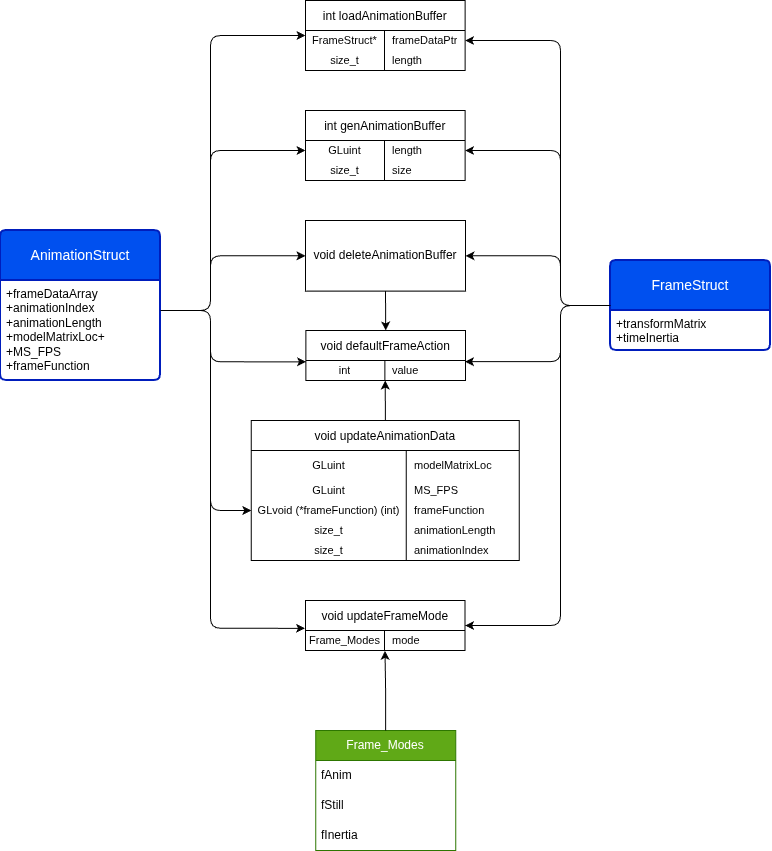
\includegraphics[width=1.0\textwidth]{figures/diagrams/libraries_animation2.png}
        \caption{Diagrama de la biblioteca de animaciones; parte 2.}
        \label{fig:graph-libraries-animation2}
    \end{subfigure}
\caption{Diagrama de la biblioteca de animaciones}
\end{figure} \label{fig:graph-libraries-animation}

\FloatBarrier
\subsection{Decisiones de diseño}

El código \ref{cod:headers-animation-libraries-1} \ref{cod:headers-animation-libraries-2} muestra el prototipo de la biblioteca en código \textit{C}.

La primera parte del diagrama \ref{fig:graph-libraries-animation1} muestra las funciones usadas para transformar la posición de la geometría: 

\begin{itemize}
    \item La estructura \textit{AnimationStruct} describe la animación: fotogramas, número de repeticiones (inercia), \textit{FPS}, etc. Para representar coordenadas, se han creado dos estructuras que describen coordenadas bidimensionales y tridimensionales.

    \item La estructura \textit{FrameStruct} describe las características de un fotograma: la matriz de transformación asociada y el tiempo de inercia, que es el número de veces que se repetirá dicha transformación.

    \item Las estructuras \textit{Coords2D} y \textit{Coords3D} almacenan coordenadas bidimensionales y tridimensionales, respectivamente, en formato decimal
    
    \item Las funciones a la izquierda modifican un \textit{buffer} local, usado más tarde para cargarlo en la animación: 
    
    \begin{enumerate}
        \item La función \textit{addScaleBuffer} agrega a un \textit{buffer} una matriz de transformación de escala.
        
        \item La función \textit{addTranslationBuffer} agrega a un \textit{buffer} una matriz de transformación de desplazamiento.
        
        \item La función \textit{addMrsBuffer} agrega a un \textit{buffer} una matriz de transformación de escala, desplazamiento y rotación, combinados.
        
        \item La función \textit{addRotateBuffer} agrega a un \textit{buffer} una matriz de transformación de rotación.
    \end{enumerate}
    
    \item Las funciones de la derecha modifican directamente la animación sin intermediario, lo que es más sencillo aunque costoso. También, debe estar configurada correctamente la animación antes de utilizarlas.
    
    \begin{enumerate}
        \item La función \textit{scaleAnimation} agrega al \textit{buffer} de animación directamente una matriz de transformación de escala.
        
        \item La función \textit{moveAnimation} agrega al \textit{buffer} de animación directamente una matriz de transformación de desplazamiento.
        
        \item La función \textit{mrsAnimation} agrega al \textit{buffer} de animación directamente una matriz de transformación de escala, desplazamiento y rotación, combinados.
        
        \item La función \textit{rotateAnimation} agrega al \textit{buffer} de animación directamente una matriz de transformación de rotación.
    \end{enumerate}
    
\end{itemize}

La segunda parte del diagrama \ref{fig:graph-libraries-animation2} muestra las funciones relacionadas a la configuración y las acciones de cada fotograma; concretamente, trata la configuración previa a la animación así como la limpieza posterior.

\begin{itemize}
    \item El enumerado, llamado \textit{Frame\_Modes}, contiene 3 estados: quieto, animación e inercia. Cuando no está en movimiento, está \textbf{quieto}; cuando está en movimiento, está en \textbf{animación}; cuando sigue repitiéndose el movimiento, está en \textbf{inercia}, hasta que para y vuelve a \textbf{quieto}.

    \item La función \textit{updateAnimationData} inicializa las propiedades de la animación almacenadas en una estructura \textit{AnimationStruct} global.

    \item El trío de funciones \textit{genAnimationBuffer}, \textit{loadAnimationBuffer} y \textit{deleteAnimationBuffer} trata el ciclo de vida de la animación: crea espacio inicial para la animación, deposita fotogramas y finalmente las destruye, respectivamente.
    
    \item La función \textit{defaultFrameAction} indica lo que ocurre en cada fotograma. Por defecto, se selecciona una función ya existente que aplica las matrices de transformación cada fotograma tantas veces como se indique en el tiempo de inercia y avanza hacia el siguiente.

    \item Finalmente, la función \textit{updateFrameMode} actualiza el estado de la animación y prepara un temporizador que activa el siguiente fotograma.
\end{itemize}

\lstinputlisting[
    float,
    floatplacement=htp,
    language=C,
    label=cod:headers-animation-libraries-1,
    caption=Prototipos de la bibliteca de animación; parte 1,
]{code/h_animation_libraries_1.h}

\lstinputlisting[
    float,
    floatplacement=htp,
    language=C,
    label=cod:headers-animation-libraries-2,
    caption=Prototipos de la biblioteca de animación; parte 2
]{code/h_animation_libraries_2.h}

\FloatBarrier
\subsection{API pública}
El usuario, según la manera en la que desee cargar los fotogramas de la animación, deberá utilizar las funciones que operan directamente sobre el \textit{buffer} de animación o las que tratan primero con un \textit{buffer} local para luego cargarlas en la animación.

En la primera opción, se asigna primero espacio en memoria al \textit{buffer} de animación y se inicializa \textit{AnimationStruct} mediante la función \textit{updateAnimationData}. Luego, se crean listas de coordenadas \textit{Coords2D} y \textit{Coords3D} para ser usadas en las transformaciones y listas de fotogramas \textit{FrameStruct}. Después, se programa la animación con las funciones \textit{add*Buffer}, cargándolas en memoria mediante \textit{loadAnimationBuffer}. Opcionalmente, puede extenderse la animación repitiendo el proceso o usando las funciones \textit{rotate|scale|moveAnimation}.

Si no se desea cargar la animación de la primera forma, sólo se modificaría la llamada a \textit{genAnimationBuffer}, indicando que el tamaño sería \textbf{cero}, y no se usarían las funciones \textit{add*Buffer} y \textit{loadAnimationBuffer}.


    \chapter{Implementación} \label{chp:implementation}

En este capítulo se describen las tecnologías empleadas en el proyecto, detalles de implementación, problemas en el desarrollo y sus soluciones, y, en general, una vista a un nivel más bajo de cada parte del diseño.

Cabe recordar que la implementación está alojada en un repositorio de \textit{Gitlab} \cite{webGitlabRenderer}.

\section{Herramientas}
Se han utilizado varias tecnologías. Se distinguirá entre tecnologías a nivel de sistema operativo, como pueden ser \textit{CMake} o \textit{git}, y tecnologías correspondientes al código directamente, como \textit{GLUT} y \textit{GLEW}.

\textbf{Tecnologías usadas a nivel de \textit{SO}:}

\begin{itemize}
    \item \textit{CMake}, para gestionar la compilación del proyecto
    \item \textit{git}, para el control de versiones del proyecto.
    \item \textit{Debian}, distribución \textit{GNU/Linux} sobre la que se ha desarrollado el proyecto.
\end{itemize}

\textbf{Tecnologías usadas a nivel de implementación y código:}

\begin{itemize}
    \item \textit{C} y \textit{C++}, como lenguaje principal de programación.
    \item \textit{OpenGL}, como \textit{API} de gráficos.
    \item \textit{GLM}, como biblioteca externa que facilita la implementación relacionada con matrices.
    \item \textit{GLUT}, como biblioteca externa que facilita la gestión de eventos específicos al sistema operativo.
    \item \textit{GLEW}, como biblioteca externa que facilita la gestión de las funciones de \textit{OpenGL}.
\end{itemize}

\section{Desarrollo de bibliotecas}
En esta sección se detallarán las bibliotecas previamente descritas en el apartado de diseño, indicando los tipos de las variables, los valores recibidos y devueltos, comportamiento y uso intencionado; todo el desarrollo se describirá según el lenguaje de programación \textit{C}.

\subsection{Shaders}
Según el diagrama de \textit{shaders} \ref{fig:graph-libraries-shader}, se crean dos funciones auxiliares que compilan y enlazan los \textit{shaders}. La función principal es \textit{loadShaders}, que compila los \textit{shaders} recibidos y los une en un programa, haciendo uso de las dos funciones anteriores.

\begin{itemize}
    \item La estructura \textit{ShaderInfo} consta de dos datos constantes: el tipo del \textit{shader}, siendo un enumerado de \textit{OpenGL} \textit{GLenum}, y la ruta hacia el fichero que contiene el \textit{shader}, siendo una cadena de caracteres \textit{char*}.

    \item La función \textit{compileShader} toma dos argumentos: Los contenidos del \textit{shader} en una cadena de caracteres \textit{GLchar*} y un tipo de \textit{shader} \textit{GLenum}. Se le indica a \textit{OpenGL} el tipo de \textit{shader} a compilar y sus contenidos, devolviendo así un número entero identificador \textit{GLuint} una vez compilado.

    \item La función \textit{linkShader} toma una lista de \textit{shaders} compilados \textit{GLuint*} y un número entero sin signo \textit{GLuint} que representa la cantidad de \textit{shaders} recibidos. Luego, se crea un programa y se enlazan a él todos los \textit{shaders} compilados. Finalmente, se devuelve el identificador \textit{GLuint} de este programa compilado.

    \item La función \textit{loadShaders} toma una lista de \textit{ShaderInfo} \textit{ShaderInfo*} y un número entero sin signo \textit{GLuint} que representa la cantidad de \textit{shaders} a procesar. Para cada \textit{shader}, lee su contenido del fichero en la ruta correspondiente y lo compila según el tipo utilizando la función \textit{compileShader}; los dos datos proporcionados por \textit{ShaderInfo}. Una vez compilados, se enlazan en un sólo programa utilizando la función \textit{linkShader}. Finalmente, se borran los \textit{shaders} que no volverán a ser utilizados y se devuelve el identificador del programa final como número entero sin signo.
\end{itemize}

\subsection{Errores}
Según el diagrama \ref{fig:graph-libraries-error}, la función principal de esta biblioteca es \textit{checkSuccess}, que recopila todos los errores y sus determinadas acciones en una instrucción \textit{switch}. Recibe la dirección a un valor y un código de error. Mediante estos dos argumentos se especifica el error y se comprueba una condición de validez distinta. Cuando es erróneo, devuelve \textit{-1}, en otro caso, \textit{0}.

\begin{itemize}
    \item Los códigos de error se reúnen en un \textit{enum} llamado \textit{Error\_Types}.
    
    \item La función \textit{checkSuccess} toma una dirección hacia un valor en memoria y un tipo de error \textit{Error\_Types}. Según el tipo del error se deduce el tipo del valor: se obtiene y se convierte al tipo deseado. Una vez se tiene el valor convertido correctamente, se comprueba con la condición del error esperada; por ejemplo, para comprobar un error cargando la animación, se valida que el valor no sea negativo. Finalmente, si hubo error se devuelve 1; en otro caso, se devuelve 0.

    \item Las macros \textit{check\_error}, \textit{check\_error\_null} y \textit{check\_error\_zero} comprueban el valor obtenido de \textit{checkSuccess} y devuelven un valor correspondiente al que indique la función mediante una instrucción \textit{return}: negativo, nulo o cero; se asume que el negativo es el valor por defecto para representar errores, por lo que no se indica en la primera función. Es particularmente útil para evitar la repetición de condicionales e instrucciones de retorno, sólo debiendo llamar a estas \textit{macros}.
    
    \item Las funciones \textit{cast\_ptr\_int} y \textit{cast\_ptr\_long} toman una dirección hacia un valor en memoria y devuelve ese mismo valor convertido en el formato correcto: \textit{int} y \textit{long}.
    
\end{itemize}

\subsection{Misceláneo}

Esta biblioteca \ref{fig:graph-libraries-miscc} recoge funciones de propósito general de \textit{C} sin usar \textit{OpenGL} ni otras bibliotecas externas.

\begin{itemize}

    \item La función \textit{readFile} es útil para obtener el código de los \textit{shader}; acepta una ruta como \textit{array} de caracteres hacia un fichero y una dirección de memoria hacia un buffer (otro puntero a memoria, es decir, un doble puntero a memoria). La función abre el fichero y lo recorre para obtener su tamaño, asigna memoria al \textit{buffer} y posteriormente vuelva el contenido del fichero en él, asegurándose de que el último byte es un carácter nulo, y se cierra el fichero.

    \item Las dos funciones restantes, \textit{create2DArray} y \textit{create2DArrayFlat}, crean un \textit{array} de dos dimensiones en dos formatos distintos: \textit{array} de \textit{arrays} (bidimensional) o un \textit{array} plano (unidimensional).

\end{itemize}

\subsection{Polígonos}

La única función actual de la biblioteca \ref{fig:graph-libraries-polygon} crea un polígono regular, en forma de un \textit{array} de vértices plano. Utilizando la ecuación paramétrica de un círculo, construye las coordenadas de cada vértice calculando los ángulos correspondientes. Esta función es especialmente útil como base de pruebas, o \textit{benchmark}, porque es sencillo estimar los triángulos que contiene un polígono regular de $n$ vértices.

El programa construye un polígono regular de $n$ vértices en el centro de la pantalla, como está detallado en la sección \ref{sec:lib-polygon}. Cualquier polígono regular es convexo \cite{webWolframConvexPolygon}, por lo cual pueden ser representados como un \textit{triangle fan} \cite[Capítulo~3]{bookOGLGuideKhronos9} y exactamente $n-2$ triángulos; en OpenGL se cambia \textit{GL\_TRIANGLES} a \textit{GL\_TRIANGLE\_FAN} en la función que dibuja el polígono. El primer vértice actúa de nodo principal y cada pareja de vértices posteriores se conecta al primero.

\subsection{Animaciones}

Esta biblioteca contiene lo necesario para crear animaciones con \textit{OpenGL}. La primera parte del diagrama \ref{fig:graph-libraries-animation1}  muestra las funciones usadas por el usuario para transformar la posición de la geometría. Las funciones a la izquierda modifican un \textit{buffer} local, usado más tarde para cargarlo en la animación. Las funciones de la derecha modifican directamente la animación sin intermediario, lo que es más sencillo aunque costoso.

\begin{itemize}

    \item La estructura \textit{FrameStruct} contiene los datos de un \textbf{fotograma}.
        \begin{enumerate}
        
            \item \textit{transformMatrix}. La matriz de transformación 4x4 de números de punto flotante que se aplica a las coordenadas de los vértices en cada fotograma
            
            \item \textit{timeInertia}. El tiempo de inercia, un número entero que indica las veces que se repetirá la transformación en los siguientes fotogramas.
            
        \end{enumerate}
    
    \item La estructura \textit{AnimationStruct} contiene los datos de la animación completa, especialmente una lista de \textit{FrameStruct}.
        \begin{enumerate}
        
            \item \textit{frameDataArray}. Una lista de fotogramas con la estructura \textit{FrameStruct}.

            \item \textit{animationIndex}. Un número entero sin signo \textit{size\_t} que representa la posición actual de la animación.

            \item \textit{animationLength}. Un número entero sin signo \textit{size\_t} que representa el tamaño de la animación.

            \item \textit{modelMatrixLoc}. Un número entero \textit{GLint} que representa la localización de la variable de tipo \textit{uniform} que almacena la matriz de transformación en el \textit{shader}.

            \item \textit{MS\_FPS}. Un número entero sin signo que representa los fotogramas por segundo transformados en milisegundos.

            \item \textit{frameFunction}. Un puntero hacia una función que acepta un argumento entero sin devolver un valor. Es el mecanismo principal del fotograma que se ejecuta por cada uno y se encarga de realizar la transición entre los estados de la animación, gestionar las matrices de transformación y la comunicación entre el programa y el \textit{shader}.
            
        \end{enumerate}
        
    \item Para representar coordenadas, se han creado dos estructuras \textit{Coords2D} y \textit{Coords3D} que almacenan coordenadas de punto flotante bidimensionales \textit{(X,Y)} y tridimensionales \textit{(X,Y,Z)}.

    \item La función \textit{extendAnimationBuffer} extiende la animación principal con fotogramas nuevos. Acepta una lista de fotogramas de tipo \textit{FrameStruct} llamada \textit{newFrames} y un tamaño de tipo \textit{size\_t} llamado \textit{length}. Se reasigna la memoria asociada al \textit{buffer} de animación principal según el nuevo tamaño, actualizando así el tamaño de la animación, y se copian los nuevos fotogramas. Es principalmente usada en las funciones de la derecha: \textit{scaleAnimation}, \textit{moveAnimation}, \textit{mrsAnimation} y \textit{rotateAnimation}.

    \item Las funciones \textit{addScaleBuffer}, \textit{addTranslationBuffer}, \textit{addRotateBuffer} y \textit{addMrsBuffer} añaden una matriz de transformación de escala, traslación, rotación o todas al mismo tiempo, respectivamente, a la lista de fotogramas en una posición \textit{index} concreta para luego ser procesados en la animación.
        \begin{itemize}
            \item Las funciones \textit{addScaleBuffer} y \textit{addTranslationBuffer} toman unas coordenadas bidimensionales de tipo \textit{Coords2D}, un número entero sin signo de veces que se repite la transformación, una lista de fotogramas de tipo \textit{FrameStruct} y un índice donde insertar la matriz en la lista de fotogramas.
        \end{itemize}

    \item Finalmente, se añadió una función \textit{centerTransformationMatrix}.
        \begin{itemize}
            \item Acepta como argumentos:
                \begin{enumerate}
                    \item Una matriz 4x4 de números flotantes.
                    \item Una lista de \textit{GLFloat} con los vértices del polígono.
                    \item Un número entero con la cantidad de vértices.
                \end{enumerate}
            \item Realiza cambios en una matriz de transformación para que rote respecto a sí mismo y no respecto al origen de coordenadas. Para ello, se hace la media de las coordenadas y se encuentra el centro del polígono, respecto al que se realizarán las transformaciones en lugar del origen de coordenadas. Puede usarse si el \textit{shader} no incorpora esta función.
        \end{itemize}
    
\end{itemize}

La segunda parte del diagrama \ref{fig:graph-libraries-animation2}  muestra las funciones relacionadas con \textit{buffers} y las acciones de cada fotograma, es decir, la configuración de la animación.

\begin{itemize}

    \item El \textit{enum} llamado \textit{Frame\_Modes} contiene 3 estados: quieto (fStill), animación (fAnim) e inercia (fInertia), útiles para representar los estados en los que se encuentra el programa.

    \item La función \textit{updateAnimationData} inicializa las propiedades de la animación almacenadas en una estructura \textit{AnimationStruct} global. Recibe como argumentos todos los valores de la estructura y se los asigna directamente a la variable global de la biblioteca.

    \item El trío de funciones \textit{genAnimationBuffer}, \textit{loadAnimationBuffer} y \textit{deleteAnimationBuffer} gestiona el ciclo de vida de la animación.
        \begin{itemize}
            \item La función \textit{genAnimationBuffer} asigna espacio inicial en memoria para la animación.
            \item La función \textit{loadAnimationBuffer} copia fotogramas en memoria. 
            \item La función \textit{deleteAnimationBuffer} las destruye liberando la memoria asignada.
        \end{itemize}
    
    \item La función \textit{defaultFrameAction} es la acción por defecto que ocurre en cada fotograma.
    
    \begin{itemize}
        \item En el estado \textit{fAnim}, se obtienen de memoria los datos del fotograma y se guardan en una variable global, se realiza una operación de multiplicación de matrices entre la matriz de inercia acumulada durante toda la animación y la matriz de transformación del fotograma actual y luego se copia a la variable \textit{uniform} del \textit{shader}. Una vez copiado el resultado, se renderiza el nuevo fotograma y se aumenta el índice de animación en uno.

        \item En el estado \textit{fInertia}, se realiza la operación entre matrices como en el estado \textit{fAnim}, aunque usando la matriz de la variable global del fotograma anterior. Se copia el resultado al \textit{shader} y se renderiza. Al final, se reduce el tiempo de inercia \textit{timeInertia} en uno.

        \item En el estado \textit{fStill} se libera la memoria del \textit{buffer} de animación y no se realiza ninguna operación.
    \end{itemize}

    % \vspace*{4\baselineskip}
    En el diagrama \ref{fig:frame-state-machine} se representa la función por defecto que se aplica cada fotograma. Cada tabla tiene como título el estado que representa y cada entrada tiene el índice y la operación que se realiza. Las flechas indican el movimiento entre estados, desde el estado origen hacia el estado destino, con un número que indica el orden que se sigue para comprobar la condición de la transición que se encuentra junto a la flecha.
    
    \begin{figure}[htp]
        \centering
        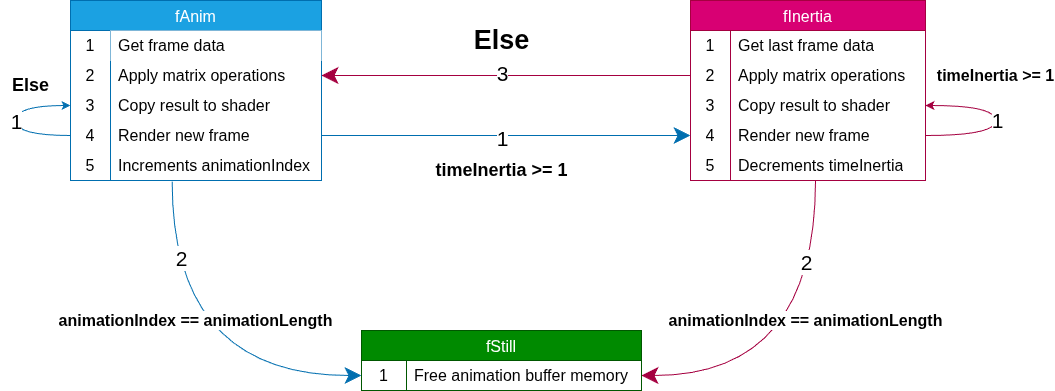
\includegraphics[width=1.0\textwidth]{figures/diagrams/frame_state_machine.png}
        \caption{Diagrama de la función por defecto por fotograma.}
        \label{fig:frame-state-machine}
    \end{figure}
    
    % \vspace*{4\baselineskip}

    \item Finalmente, la función \textit{updateFrameMode} actualiza el estado de la animación y prepara un temporizador que activa el siguiente fotograma.
    
\end{itemize}

\FloatBarrier
\subsection{Ejemplo de uso}

Con el objetivo de ilustrar la cooperación entre las diferentes bibliotecas creadas, se diseñará un programa de ejemplo, a alto nivel, cuyo propósito sea crear una animación con un polígono regular. El objetivo es generar matrices de transformación que se enviarán al \textit{shader} en forma de variable \textit{uniform}.

El programa está representado a alto nivel en el diagrama \ref{fig:example-program-diagram}. Los rectángulos coloreados son los que incluyen funcionalidades de las bibliotecas. Aunque no representado para simplificar el diagrama, se utiliza la comprobación de errores de la biblioteca cuando sea posible en todo el programa.

\begin{figure}[htp]
    \centering
    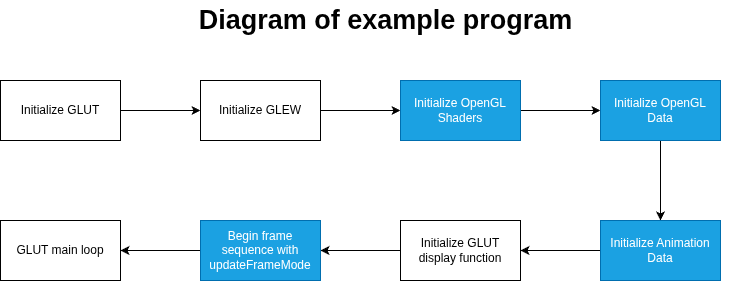
\includegraphics[width=1.0\textwidth]{figures/diagrams/example_program_diagram.png}
    \caption{Diagrama del programa de ejemplo.}
    \label{fig:example-program-diagram}
\end{figure}

\FloatBarrier

A continuación, se describe la rutina de inicialización de \textit{shaders} y cómo se usa la biblioteca para procesarlos y crear un programa. Primero, se crea un \textit{array} de tipo \textit{ShaderInfo} de una longitud del número de \textit{shaders} a procesar, con el tipo de \textit{shader} y la ruta hacia el fichero con su contenido. Este \textit{array} es recibido por la función \textit{loadShaders} y éste genera el \textbf{programa} ya procesado. Se obtiene la localización de la variable \textit{uniform} que contiene la matriz de transformación y se activa el programa.

Además del código del programa escrito en \textit{C}, es necesario escribir los \textit{shaders} correspondientes en la ruta \textit{/shaders} del proyecto; la extensión \textit{.vert} y \textit{.frag} son pertenecientes a los \textit{shaders} \textit{vertex} y \textit{fragment}.

\begin{itemize}
    \item El \textit{vertex shader} es responsable de realizar la operación matricial que modifica la posición del vértice.
        \begin{enumerate}
            
            \item Contiene un vector bidimensional llamado \textbf{vPosition} que contiene las coordenadas del vértice y una matriz 4x4 \textit{uniform} de tipo \textit{mat4} llamada \textbf{modelMatrix} que contiene la matriz de transformación.

            \item Se crea una matriz 4x4 llamada \textit{centerMatrix} que multiplica a \textit{modelMatrix} para que realice la transformación entorno a sí mismo.

            \item Finalmente, se multiplican las coordenadas del vértice a la matriz de transformación centrada y se obtiene la nueva posición del vértice \textit{gl\_Position}.

        \end{enumerate}

    \item El \textit{fragment shader} es un \textit{shader} simple que asigna el color blanco a \textit{fragColor}, que es un vector de 4 dimensiones.
\end{itemize}

\begin{figure}[htp]
    \centering
    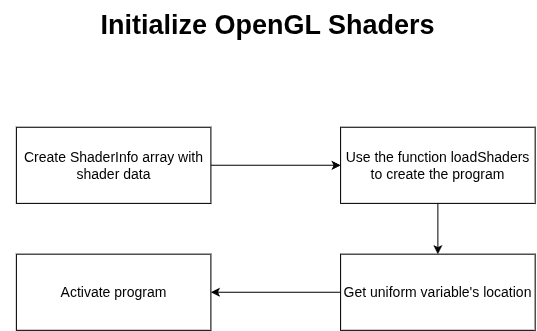
\includegraphics[width=0.8\textwidth]{figures/diagrams/example_program_shader.png}
    \caption{Diagrama de inicialización de shaders en el programa de ejemplo.}
    \label{fig:example-program-shaders}
\end{figure}

\FloatBarrier

El diagrama \ref{fig:example-program-gl-data} representa el proceso para crear los datos que usará \textit{OpenGL} para dibujar la geometría.

\begin{enumerate}

    \item Se crea un polígono regular mediante la función de la biblioteca de polígonos \textit{createNGonVertices}, indicando el número de vértices deseados, sus coordenadas, dimensiones y el \textit{buffer} donde se almacenarán los vértices del polígono.

    \item Deberán crearse los \textit{buffers} de \textit{OpenGL}, los cuales en este caso son el \textit{VAO} y el \textit{VBO}, mediante el par de funciones (para cada objeto) \textit{glGenVertexArrays} y \textit{glBindVertexArray}; generan internamente el objeto y luego lo vincula.

    \item Luego, se almacenan los vértices en el \textit{VBO} mediante la función \textit{glBufferData}, indicando el tipo de \textit{buffer}, el tamaño en \textit{bytes} a copiar, el origen y el tipo de uso que en este caso sería \textit{GL\_DYNAMIC\_DRAW}.

    \item Después, se especifican las posiciones de los atributos de los vértices con \textit{glVertexAttribPointer} y se activan con \textit{glEnableVertexAttribArray}.

    \item También, se inicializa la variable \textit{uniform} en el \textit{shader} que se utiliza para la matriz de transformación con una matriz de identidad.

    \item Finalmente, se libera el \textit{buffer} de vértices creado inicialmente para alojar el polígono.

\end{enumerate}

\begin{figure}[htp]
    \centering
    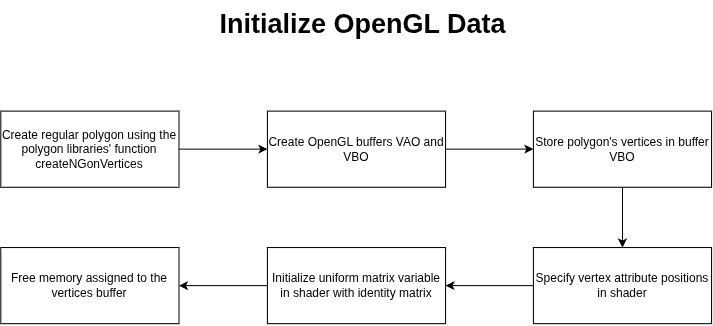
\includegraphics[width=1.0\textwidth]{figures/diagrams/example_program_gl_data.png}
    \caption{Diagrama de inicialización de datos para OpenGL.}
    \label{fig:example-program-gl-data}
\end{figure}

\FloatBarrier

Finalmente, se muestra la inicialización de los datos de animación en la figura \ref{fig:example-program-animation}.

\begin{figure}[htp]
    \centering
    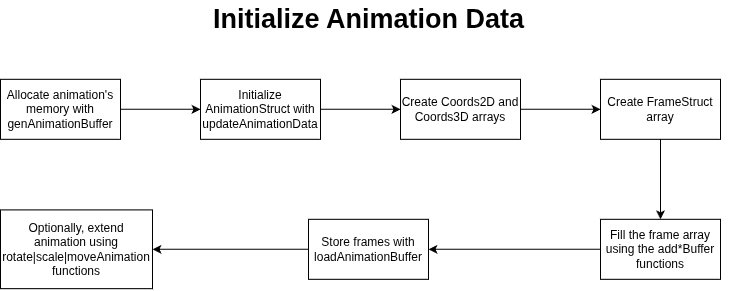
\includegraphics[width=1.0\textwidth]{figures/diagrams/example_program_animation.png}
    \caption{Diagrama de inicialización de los datos para la animación.}
    \label{fig:example-program-animation}
\end{figure}

\begin{enumerate}
    \item Primero, se asigna memoria para el \textit{buffer} de animación con \textit{genAnimationBuffer}, indicando el tamaño en \textit{bytes} y el número de elementos.

    \item Luego, se actualizan los atributos de la estructura de datos \textit{AnimationStruct} mediante la función \textit{updateAnimationData}, que recibe como argumentos las propiedades y se las asigna.

    \item Se crean, también, dos \textit{arrays} para coordenadas bidimensionales \textit{Coords2D} y tridimensionales \textit{Coords3D} para usar en las transformaciones.

    \item Se crea un \textit{buffer} de fotogramas, que se completará usando funciones del tipo \textit{add*Buffer}, declaradas en la biblioteca de animación; estas funciones añaden fotogramas \textit{FrameStruct} a un \textit{buffer}, indicando el tipo de transformación, sus características y el índice en el que colocar el fotograma.

    \item Una vez lleno el \textit{buffer} de fotogramas, se guardan en memoria con \textit{loadAnimationBuffer}.

    \item Opcionalmente, puede extenderse la animación usando las funciones \textit{rotate|scale|moveAnimation}, indicando las características de la transformación y el fotograma, que automáticamente colocan la transformación correspondiente en la secuencia de animación.
\end{enumerate}

\subsection{Demostración}
En las subfiguras de la figura \ref{fig:test-animation} se encuentran capturas de pantalla realizadas durante la animación.

\begin{figure}[htp]
    \centering
    \begin{subfigure}[t]{0.3\textwidth}
        
\includegraphics[width=\textwidth]{figures/evidence/test_animation_still.png}
        \caption{Polígono parado.}
        \label{fig:test-animation-still}
    \end{subfigure}
    \hfill
    \begin{subfigure}[t]{0.3\textwidth}
        \centering
        
\includegraphics[width=\textwidth]{figures/evidence/test_animation_move.png}
        \caption{Polígono en movimiento.}
        \label{fig:test-animation-move}
    \end{subfigure}
    \hfill
    \begin{subfigure}[t]{0.3\textwidth}
        \centering
        
\includegraphics[width=\textwidth]{figures/evidence/test_animation_rotate_1.png}
        \caption{Polígono rotando entorno al eje y.}
        \label{fig:test-animation-rotate-1}
    \end{subfigure}
    \hfill
    \begin{subfigure}[t]{0.3\textwidth}
        \centering
        
\includegraphics[width=\textwidth]{figures/evidence/test_animation_rotate_2.png}
        \caption{Polígono rotando entorno al eje x.}
        \label{fig:test-animation-rotate-2}
    \end{subfigure}
    \hfill
    \begin{subfigure}[t]{0.3\textwidth}
        \centering
        
\includegraphics[width=\textwidth]{figures/evidence/test_animation_rotate_3.png}
        \caption{Polígono rotando entorno al eje z.}
        \label{fig:test-animation-rotate-3}
    \end{subfigure}
    \hfill
    \begin{subfigure}[t]{0.3\textwidth}
        \centering
        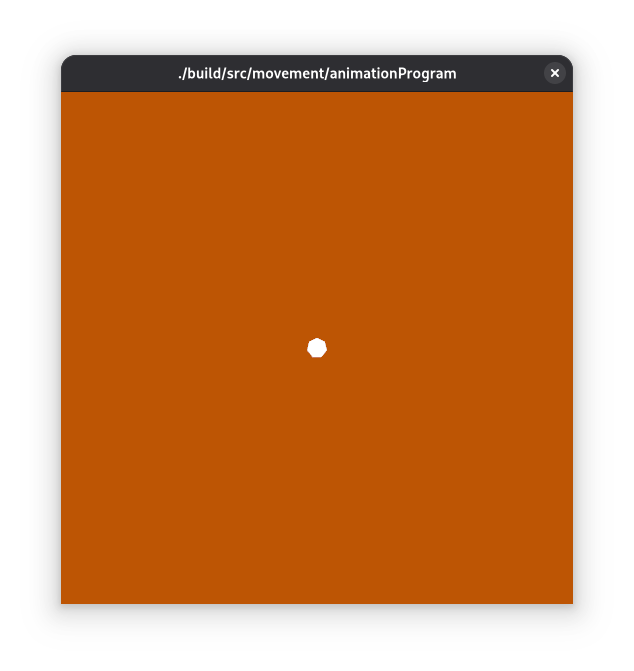
\includegraphics[width=\textwidth]{figures/evidence/test_animation_scale.png}
        \caption{Polígono encogiendo.}
        \label{fig:test-animation-scale}
    \end{subfigure}

\end{figure} \label{fig:test-animation}

\section{Conclusiones}
En esta sección se ha explorado con detalle las bibliotecas y las funciones y estructuras que las componen. También, se ha ofrecido un ejemplo de uso con el objetivo de que el lector pueda encajar las diferentes partes del proyecto y conceptualizar un resultado.

    \chapter{Pruebas} \label{chp:tests}

\section{Introducción}

\textbf{Las optimizaciones utilizadas durante las pruebas fueron las provocadas por la \textit{flag} \textit{O3}} en el compilador \textit{GCC} \cite{webGccOptimizationOptions}.

En este capítulo se describen las pruebas realizadas sobre los programas desarrollados en el proyecto, así como el análisis de los resultados desde diferentes perspectivas, con el fin de evaluar aspectos como los valores de las métricas obtenidas, la uniformidad de los resultados, el comportamiento general y el rendimiento. Para ello, las versiones empleadas en las pruebas incorporan código adicional específico para caracterizar el rendimiento, generando dos ficheros: \textit{.log}, que recoge información legible para el usuario, y \textit{.dat}, que contiene los datos necesarios para la representación gráfica. Para las pruebas de rendimiento de vértices en un polígono \ref{sec:polygon-performance-test} y de animación \ref{sec:animation-performance-test}, los ficheros \textit{.dat} son procesados mediante \textit{gnuplot} y genera las gráficas correspondientes.

Se han realizado pruebas sobre el uso de memoria \ref{sec:memory-analysis} con \textit{Valgrind} \cite{webValgrind}.

También, se ha realizado un análisis más profundo de \textit{CPU} \ref{sec:cpu-analysis} con \textit{perf} \cite{webPerf}.

Las pruebas se han ejecutado en el siguiente entorno \textit{hardware} y \textit{software}:

\begin{itemize}

    \item El sistema operativo es una distribución de \textit{GNU/Linux}, concretamente, \textit{Debian 13, Trixie} \cite{webDebian}.
    
    \item La \textit{CPU} es \textit{Intel(R) Core(TM) i5-7400 (4) @ 3.50 GHz}.

    \item La \textit{GPU} es \textit{NVIDIA GeForce GTX 1050 [Discrete]}.

    \item La versión de \textit{OpenGL} es: 4.6.0 NVIDIA 550.163.01.

    \item La versión del compilador \textit{gcc} es gcc (Debian 14.2.0-19) 14.2.0.

    \item La versión de \textit{make} es GNU Make 4.4.1.
    
\end{itemize}

\section{Pruebas de rendimiento de creación de polígonos} \label{sec:polygon-performance-test}

La prueba diseñada para probar el rendimiento de la creación de polígonos con una alta cantidad de vértices ha sido realizar iteraciones en un bucle en el que se aumenta progresivamente su número, y se analiza el rendimiento del programa.

El funcionamiento del núcleo del programa, sin profundizar en configuración ni otros mecanismos ya explicados anteriormente y no relevantes para la prueba, es muy simple: en un bucle, con un número determinado de vértices inicial, crea un polígono regular de ese número de vértices que luego se renderiza. En la siguiente iteración, se realiza la misma operación con un vértice más. 

\subsection{Problemas encontrados}
En la prueba de los vértices de un polígono el principal problema fue cómo visualizar la evolución del rendimiento al incrementar progresivamente los vértices de un polígono. Finalmente, se decidió desarrollar un único programa que cada fotograma aumente el número de vértices y renderice el polígono de nuevo.

Una vez realizada la prueba era necesario medir los tiempos y escribir los registros. Se crearon dos tipos de fichero para este propósito: uno que registra datos en crudo para las gráficas y otro más legible para el usuario. El mayor inconveniente era el dónde situar estas medidas, y entonces se decidió medir la creación del polígono y la renderización del mismo que realizan la funciones \textit{initGLData} y \textit{display}; este es el comportamiento de la \textit{CPU} y la \textit{GPU}, respectivamente.

\FloatBarrier
\subsection{Resultados}

Se muestra una captura de pantalla tomada durante la prueba \ref{fig:test-polygon-1000}.

\begin{figure}[htp]
    \centering
    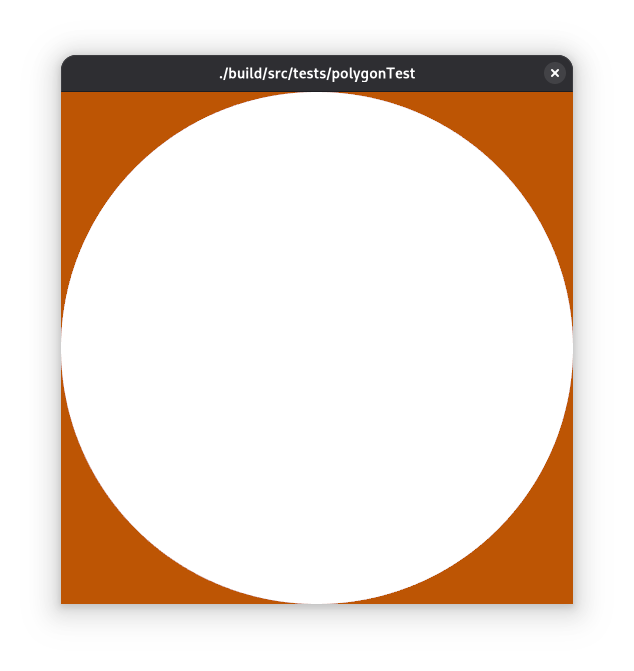
\includegraphics[width=1.0\textwidth]{figures/evidence/test_polygon_1000.png}
    \caption{Captura de pantalla de la prueba del polígono de 3 a 1000 vértices}
    \label{fig:test-polygon-1000}
\end{figure}


Utilizando los datos generados por la prueba se han creado varias gráficas que representan el rendimiento de la \textit{CPU} y la \textit{GPU} durante la ejecución. La primera gráfica representa el coste temporal que requiere crear los polígonos cuyos vértices aumentan progresivamente, desde \textbf{3} hasta \textbf{1000}, y la segunda y tercera gráfica representan la \textit{CPU} y la \textit{GPU} durante la renderización.

Observando la gráfica \ref{fig:polygon-graph-vertices}, se puede deducir a simple vista que es lineal. Con los resultados de diferentes medidas realizadas sobre estos datos en la tabla \ref{tbl:results-polygon-vertices} puede resaltarse:

\begin{itemize}

    \item Dado que $media > mediana > moda$, se deduce que los datos están sesgados positivamente y se acumulan hacia la izquierda de la gráfica.

    \item La desviación estándar y la varianza grandes indican que los datos difieren de la media bastante: que la varianza esté cerca de la mitad de la escala no es coincidencia, ya que la gráfica sigue una distribución lineal.

    \item El valor del \textit{IQR} confirma la anterior deducción: los datos en el medio de la gráfica tienen una dispersión del $3.43$, que es aproximado a la mitad de la escala.
    
    \item La correlación entre los datos de vértices y el tiempo de \textit{CPU} es cercana a $1$: siendo el crecimiento del número de vértices lineal, también lo sería el rendimiento.

\end{itemize}

\FloatBarrier

\begin{figure}[htp]
    \centering
    \includesvg[inkscapelatex=false, width=1.0\textwidth]{figures/graphs/polygon_graphs_vertices.svg}
    \caption{Gráfica que representa el rendimiento de la \textit{CPU} en la prueba del polígono durante su creación.}
    \label{fig:polygon-graph-vertices}
\end{figure}

\begin{table}[htp]
\centering

    % Esta primera línea define las columnas de la tabla. Los posibles tipos de columna son:
    % c: texto centrado
    % l: texto alineado a la izquierda
    % r: texto centrado a la derecha
    % p: columna de ancho fijo
    % Las columnas tienen ancho dinámico según la anchura máxima de los elementos que contengan.

    % Las columnas l/r/c no parten el texto en filas diferentes si éste es demasiado largo. Para ello, puede utilizar el tipo de columna de ancho fijo "p".
    
    % Las barras verticales | se usan para definir los bordes verticales de la tabla. Pruebe a eliminar algunas y observe qué ocurre.
    \begin{center}
    \begin{tabular}{ | l | l | }
        
        % A continuación van las filas de la tabla. En cada fila, las columnas se separan con el carácter &
        % Para terminar una fila se usa \\
        % Para incluir un borde horizontal entre filas se usa \hline
        
        % Cabecera con textos en negrita:
        \hline
        \textbf{Media: }  & 3.203347 \\
        \hline
        \textbf{Mediana} & 2.975000 \\
        \hline
        \textbf{Moda} & 2.518307 \\
        \hline
        \textbf{IQR} & 3.437500 \\
        \hline
        \textbf{Varianza} & 3.822103 \\
        \hline
        \textbf{Desviación estándar} & 1.955020 \\
        \hline
        \textbf{Covarianza (v)} & 561.004122 \\
        \hline
        \textbf{Correlación (v)} & 0.995537 \\
        \hline
        \textbf{Q1} & 1.5425 \\
        \hline
        \textbf{Q2} & 2.9750 \\
        \hline
        \textbf{Q2} & 4.9800 \\
        \hline
        
    \end{tabular} 
    \end{center}
    
    \caption{Resultados de la creación de vértices en la prueba del polígono}
    \label{tbl:results-polygon-vertices} 
\end{table}

\FloatBarrier

El par de gráficas \ref{fig:polygon-graphs-render} representan el rendimiento durante la renderización por parte de la \textit{GPU} y la \textit{CPU}. Las dos gráficas muestran un comportamiento logarítmico, aunque la primera se ajusta más a una función como $log(x)$ y la segunda como $log(log(x))$. Pueden observarse en los resultados de la \textit{GPU} \ref{tbl:results-polygon-render-gpu}:

\begin{itemize}

    \item La desviación estándar es muy pequeña respecto a los datos, lo que quiere decir que el \textit{jittering} es mínimo y los los datos no difieren mucho respecto a la media. 
    
    \item Dado que $media > mediana > moda$, se deduce que los datos están sesgados negativamente y se acumulan hacia la izquierda de la gráfica.
    
    \item La covarianza mayor a $0$ entre la \textit{CPU} y los vértices indica una dependencia entre los datos positiva.
    
    \item La correlación entre la \textit{CPU} y los vértices está entre $0$ y $1$, aunque acercándose a este último. Esto indica una relación positiva y lineal entre estas dos variables.
    
    \item Los cálculos de covarianza y correlación cercanos a $0$ entre la \textit{CPU} y la \textit{GPU} indican que los dos datos son independientes y no hay relación entre ellas.

\end{itemize}

\FloatBarrier
\begin{figure}[htp]
    \centering
    \includesvg[inkscapelatex=false, width=1.0\textwidth]{figures/graphs/polygon_graphs_render.svg}
    \caption{Gráficas que representan el rendimiento de la \textit{GPU} y la \textit{CPU} en la prueba del polígono durante la renderización.}
    \label{fig:polygon-graphs-render}
\end{figure}

\begin{table}[htp]
\centering

    % Esta primera línea define las columnas de la tabla. Los posibles tipos de columna son:
    % c: texto centrado
    % l: texto alineado a la izquierda
    % r: texto centrado a la derecha
    % p: columna de ancho fijo
    % Las columnas tienen ancho dinámico según la anchura máxima de los elementos que contengan.

    % Las columnas l/r/c no parten el texto en filas diferentes si éste es demasiado largo. Para ello, puede utilizar el tipo de columna de ancho fijo "p".
    
    % Las barras verticales | se usan para definir los bordes verticales de la tabla. Pruebe a eliminar algunas y observe qué ocurre.
    \begin{center}
    \begin{tabular}{ | l | l | }
        
        % A continuación van las filas de la tabla. En cada fila, las columnas se separan con el carácter &
        % Para terminar una fila se usa \\
        % Para incluir un borde horizontal entre filas se usa \hline
        
        % Cabecera con textos en negrita:
        \hline
        \textbf{Media: }  & 0.118084 \\
        \hline
        \textbf{Mediana} & 0.123392 \\
        \hline
        \textbf{Moda} & 0.134008 \\
        \hline
        \textbf{IQR} & 0.040960 \\
        \hline
        \textbf{Varianza} & 0.001664 \\
        \hline
        \textbf{Desviación estándar} & 0.040793 \\
        \hline
        \textbf{Covarianza (v)} & 7.548455 \\
        \hline
        \textbf{Correlación (v)} & 0.641963 \\
        \hline
        \textbf{Covarianza (GPU)} & 0.001354 \\
        \hline
        \textbf{Correlación (GPU)} & 0.759181 \\
        \hline
        \textbf{Q1} & 0.098304 \\
        \hline
        \textbf{Q2} & 0.123392 \\
        \hline
        \textbf{Q3} & 0.139264 \\
        \hline
        
    \end{tabular} 
    \end{center}
    
    \caption{Resultados de la renderización en la prueba del polígono: \textbf{GPU}}
    
    \label{tbl:results-polygon-render-gpu}
\end{table}
\FloatBarrier

Pueden observarse en los resultados de la \textit{CPU} \ref{tbl:results-polygon-render-cpu}:
\begin{itemize}

    \item La varianza y desviación típica son mayores que en las de la \textit{GPU} y son relativamente grandes respecto a la escala de los datos. Esto indica una alta dispersión en los resultados respecto a la media.

    \item El \textit{IQR} es cercano a 0, lo que indica una similitud entre cuartiles y, a su vez, mínima diferencia en los resultados.

    \item La covarianza entre la \textit{CPU} y los vértices indica una dependencia negativa entre estas dos variables: cuando aumentan los vértices, disminuye la duración de la \textit{CPU}.

    \item La correlación entre la \textit{CPU} y los vértices es cercana a $0$, lo que indica que existe independencia lineal entre estas dos variables.

    \item Los cálculos de covarianza y correlación cercanos a $0$ entre la \textit{CPU} y la \textit{GPU} indican que los dos datos son independientes y no hay relación entre ellas.

\end{itemize}

\FloatBarrier
\begin{table}[htp]
\centering

    % Esta primera línea define las columnas de la tabla. Los posibles tipos de columna son:
    % c: texto centrado
    % l: texto alineado a la izquierda
    % r: texto centrado a la derecha
    % p: columna de ancho fijo
    % Las columnas tienen ancho dinámico según la anchura máxima de los elementos que contengan.

    % Las columnas l/r/c no parten el texto en filas diferentes si éste es demasiado largo. Para ello, puede utilizar el tipo de columna de ancho fijo "p".
    
    % Las barras verticales | se usan para definir los bordes verticales de la tabla. Pruebe a eliminar algunas y observe qué ocurre.
    \begin{center}
    \begin{tabular}{ | l | l | }
        
        % A continuación van las filas de la tabla. En cada fila, las columnas se separan con el carácter &
        % Para terminar una fila se usa \\
        % Para incluir un borde horizontal entre filas se usa \hline
        
        % Cabecera con textos en negrita:
        \hline
        \textbf{Media}  & 0.132385 \\
        \hline
        \textbf{Mediana} & 0.130000 \\
        \hline
        \textbf{Moda} & 0.125230 \\
        \hline
        \textbf{IQR} & 0.010000 \\
        \hline
        \textbf{Varianza} & 0.001912 \\
        \hline
        \textbf{Desviación estándar} & 0.043723 \\
        \hline
        \textbf{Covarianza (v)} & 3.647974 \\
        \hline
        \textbf{Correlación (v)} & 0.289460 \\
        \hline
        \textbf{Covarianza (GPU)} & 0.001354 \\
        \hline
        \textbf{Correlación (GPU)} & 0.759181 \\
        \hline
        \textbf{Q1} & 0.13 \\
        \hline
        \textbf{Q2} & 0.13 \\
        \hline
        \textbf{Q3} & 0.14 \\
        \hline
        
    \end{tabular} 
    \end{center}
    
    \caption{Resultados de la renderización en la prueba del polígono: \textbf{CPU}}
    
    \label{tbl:results-polygon-render-cpu}
\end{table}

\section{Pruebas de rendimiento de animaciones} \label{sec:animation-performance-test}

Esta prueba se ha realizado con $2^{10}$ polígonos de \textbf{32} lados, o también llamados \textbf{icosidodecágonos}, desplegados por la pantalla. Para conseguir un escenario sencillo y previsible sobre la prueba, se decidió agrupar los polígonos en una matriz cuadrada y siempre la cantidad siendo $2^x$, donde $x$ es un número par con el objetivo de construir una matriz cuadrada de tamaño $2^{(x/2)}$ por $2^{(x/2)}$. Cada polígono obtiene sus coordenadas en función del número de polígonos a crear y de las dimensiones de la ventana. El diámetro de cada polígono se calcularía entonces como $\frac{1}{P}$, siendo $P$ el número de polígonos por fila o columna, para que cubran toda la ventana sin colisionar entre ellos, calculado como $P = 2^{\frac{M}{2}}$; Luego, considerando que en \textit{OpenGL} el origen de coordenadas está en el centro: $(x,y) = (-\frac{1}{2} + r + d \times i, \frac{1}{2} - (r + d \times j))$. El diámetro de cada polígono $d$ se calcula de manera inversamente proporcional a $P$: $d = \frac{1}{p}$. De esta forma, se coloca cada polígono en cada casilla de la matriz. Con estas coordenadas calculadas, puede llamarse a la función \textit{createNGonVertices} para crear el polígono regular.

\begin{algorithm}
\caption{Algoritmo de creación de polígonos en matriz cuadrada}\label{alg:polygon-matrix}
\begin{algorithmic}

\Require $M$ is \textbf{pair} and $N >0$ \Comment{$N$ is the number of vertices of each polygon}
\State $P \gets 2^{\frac{M}{2}}$ \Comment{$P$ is the number of polygons per row or column}
\State $d \gets \frac{1}{P}$ \Comment{$d$ is the diameter of each polygon}
\State $r \gets \frac{d}{2}$
\While{$j < P$}
    \While{$i < P$}
        \State $x \gets -\frac{1}{2} + r + d \times i$
        \State $y \gets \frac{1}{2} - (r + d \times j)$
        \newline
        \texttt{createNGonVertices($N$, $x$, $y$, $r$, \&(vertices[$P \times j + i$]))}
    \EndWhile
\EndWhile

\end{algorithmic}
\end{algorithm}

\subsection{Problemas encontrados}
En la prueba de animación, el principal problema residía en la naturaleza de la prueba a realizar; la cual consistía en reproducir una animación donde la mayor cantidad de polígonos actuaran a la vez en una misma escena, moviéndose al unísono, para comprobar cómo afectaría eso al rendimiento. Para poder representar todos estos polígonos a la vez y que fueran visibles, era necesario agruparlos correctamente y que no ocultasen unos a otros. Entonces, se calcularon las coordenadas de cada polígono como si de una matriz se tratase y cada figura un elemento de ella, con unos márgenes entre ellos para separarlos mínimamente. 

En esta prueba la posición en la que colocar las mediciones de tiempo era menos intuitiva. Ya que el objetivo principal era medir el rendimiento de la \textit{GPU}, se mide el tiempo entre fotogramas; asimismo, el rendimiento de la \textit{CPU} se mide en el mismo intervalo para poder comparar. También, fue útil medir el tiempo que tardaba la \textit{CPU} en crear todos los polígonos usados en la animación.

\subsection{Resultados}

Se muestra una captura de pantalla de la prueba de animación en funcionamiento \ref{fig:test-animation-1024}.

\begin{figure}[htp]
    \centering
    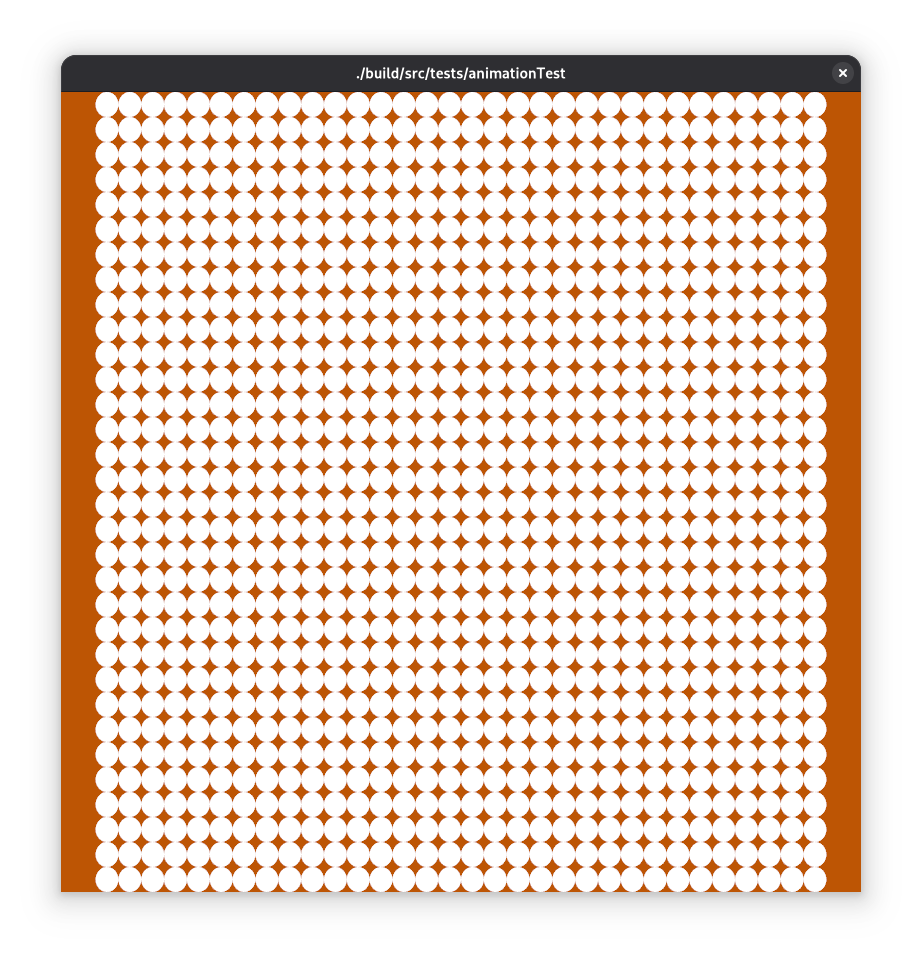
\includegraphics[width=1.0\textwidth]{figures/evidence/animation_1024.png}
    \caption{Captura de pantalla de la prueba de la animación de 1024 polígonos en una matriz cuadrada.}
    \label{fig:test-animation-1024}
\end{figure}

Los resultados de la \textit{CPU} \ref{fig:animation-graph-polygon} durante la creación de polígonos indican simetría y mínima dispersión:

\begin{itemize}

\item Dado que $media < mediana < moda$, se puede deducir que la distribución de los datos está sesgada negativamente y se acumulan ligeramente hacia la izquierda.

\item El \textit{IQR} calculado a partir de los cuartiles indica que la dispersión de los valores en la mitad de la gráfica tienen una dispersión de $0.03$, lo que es despreciable en esta escala.

\item Los valores de la variación y la desviación estándar son pequeños, lo que indica poca dispersión respecto a la media.

\end{itemize}

\FloatBarrier
\begin{figure}[htp]
    \centering
    \includesvg[inkscapelatex=false, width=1.0\textwidth]{figures/graphs/animation_graphs_polygon.svg}
    \caption{Gráfica que representa el rendimiento de la \textit{CPU} en la prueba de animación durante la creación de los polígonos.}
    \label{fig:animation-graph-polygon}
\end{figure}

\begin{table}[htp]
\centering

    % Esta primera línea define las columnas de la tabla. Los posibles tipos de columna son:
    % c: texto centrado
    % l: texto alineado a la izquierda
    % r: texto centrado a la derecha
    % p: columna de ancho fijo
    % Las columnas tienen ancho dinámico según la anchura máxima de los elementos que contengan.

    % Las columnas l/r/c no parten el texto en filas diferentes si éste es demasiado largo. Para ello, puede utilizar el tipo de columna de ancho fijo "p".
    
    % Las barras verticales | se usan para definir los bordes verticales de la tabla. Pruebe a eliminar algunas y observe qué ocurre.
    \begin{center}
    \begin{tabular}{ | l | l | }
        
        % A continuación van las filas de la tabla. En cada fila, las columnas se separan con el carácter &
        % Para terminar una fila se usa \\
        % Para incluir un borde horizontal entre filas se usa \hline
        
        % Cabecera con textos en negrita:
        \hline
        \textbf{Media: }  & 0.202725 \\
        \hline
        \textbf{Mediana} & 0.210000 \\
        \hline
        \textbf{Moda} & 0.224551 \\
        \hline
        \textbf{IQR} & 0.030000 \\
        \hline
        \textbf{Varianza} & 0.000965 \\
        \hline
        \textbf{Desviación estándar} & 0.031060 \\
        \hline
        \textbf{Q1} & 0.19 \\
        \hline
        \textbf{Q2} & 0.21 \\
        \hline
        \textbf{Q3} & 0.22 \\
        \hline
        
    \end{tabular} 
    \end{center}
    
    \caption{Resultados de la creación de polígonos en la prueba de animación (\textbf{CPU})}
    
    \label{table:results-animation-polygons}
\end{table}

\FloatBarrier

Pueden observarse en los resultados de la \textit{CPU}:
\begin{itemize}

    \item Dado que $media > mediana > moda$, se deduce que los datos están sesgados positivamente y se acumulan hacia la izquierda de la gráfica.

    \item Los valores de la varianza y la desviación típica son muy pequeños, lo que indica que los datos difieren muy ligeramente de la media.

    \item El \textit{IQR} con valor $0.047$ indica que la dispersión de los valores en la mitad de la gráfica es diminuta y su distribución es uniforme.

    \item La covarianza entre la \textit{CPU} y los vértices indica una dependencia negativa entre estas dos variables: cuando aumentan los vértices, disminuye la duración de la \textit{CPU}.

    \item La correlación entre la \textit{CPU} y los vértices es cercana a $0$, lo que indica que existe independencia lineal entre estas dos variables.

    \item Los cálculos de covarianza y correlación cercanos a $0$ entre la \textit{CPU} y la \textit{GPU} indican que los dos datos son independientes y no hay relación entre ellas.

\end{itemize}

La gráfica de la \textit{GPU} \ref{fig:animation-graphs-render} es interesante, ya que pueden distinguirse los distintos estados por los que pasa la animación: rotación, escala y traslación. Estos tres estados se ven reflejados en la gráfica con líneas en forma de \textit{zigzag} para la rotación, una línea recta para la traslación y una semiesfera para la escala (hacia abajo cuando se encoge y hacia arriba cuando se agranda). Sin embargo, la gráfica de la \textit{CPU} es constante, aunque con datos dispersos por la espera de sincronización entre los componentes.

\begin{figure}[htp]
    \centering
    \includesvg[inkscapelatex=false, width=1.0\textwidth]{figures/graphs/animation_graphs_render.svg}
    \caption{Gráficas que representan el rendimiento de la \textit{GPU} y la \textit{CPU} en la prueba de animación durante la renderización.}
    \label{fig:animation-graphs-render}
\end{figure}

\FloatBarrier

\begin{table}[htp]
\centering

    % Esta primera línea define las columnas de la tabla. Los posibles tipos de columna son:
    % c: texto centrado
    % l: texto alineado a la izquierda
    % r: texto centrado a la derecha
    % p: columna de ancho fijo
    % Las columnas tienen ancho dinámico según la anchura máxima de los elementos que contengan.

    % Las columnas l/r/c no parten el texto en filas diferentes si éste es demasiado largo. Para ello, puede utilizar el tipo de columna de ancho fijo "p".
    
    % Las barras verticales | se usan para definir los bordes verticales de la tabla. Pruebe a eliminar algunas y observe qué ocurre.
    \begin{center}
    \begin{tabular}{ | l | l | }
        
        % A continuación van las filas de la tabla. En cada fila, las columnas se separan con el carácter &
        % Para terminar una fila se usa \\
        % Para incluir un borde horizontal entre filas se usa \hline
        
        % Cabecera con textos en negrita:
        \hline
        \textbf{Media: }  & 0.206815 \\
        \hline
        \textbf{Mediana} & 0.192512 \\
        \hline
        \textbf{Moda} & 0.163906 \\
        \hline
        \textbf{IQR} & 0.047104 \\
        \hline
        \textbf{Varianza} & 0.002715 \\
        \hline
        \textbf{Desviación estándar} & 0.052101 \\
        \hline
        \textbf{Covarianza (GPU)} & 0.000971 \\
        \hline
        \textbf{Correlación (GPU)} & 0.419512 \\
        \hline
        \textbf{Q1} & 0.190464 \\
        \hline
        \textbf{Q2} & 0.192512 \\
        \hline
        \textbf{Q3} & 0.237568 \\
        \hline
        
    \end{tabular} 
    \end{center}
    
    \caption{Resultados de la renderización en la prueba del polígono: \textbf{GPU}}
    
    \label{table:results-animation-render-gpu}
\end{table}
\begin{table}[htp]
\centering

    % Esta primera línea define las columnas de la tabla. Los posibles tipos de columna son:
    % c: texto centrado
    % l: texto alineado a la izquierda
    % r: texto centrado a la derecha
    % p: columna de ancho fijo
    % Las columnas tienen ancho dinámico según la anchura máxima de los elementos que contengan.

    % Las columnas l/r/c no parten el texto en filas diferentes si éste es demasiado largo. Para ello, puede utilizar el tipo de columna de ancho fijo "p".
    
    % Las barras verticales | se usan para definir los bordes verticales de la tabla. Pruebe a eliminar algunas y observe qué ocurre.
    \begin{center}
    \begin{tabular}{ | l | l | }
        
        % A continuación van las filas de la tabla. En cada fila, las columnas se separan con el carácter &
        % Para terminar una fila se usa \\
        % Para incluir un borde horizontal entre filas se usa \hline
        
        % Cabecera con textos en negrita:
        \hline
        \textbf{Media}  & 0.177133 \\
        \hline
        \textbf{Mediana} & 0.170000 \\
        \hline
        \textbf{Moda} & 0.155733 \\
        \hline
        \textbf{IQR} & 0.000000 \\
        \hline
        \textbf{Varianza} & 0.001975 \\
        \hline
        \textbf{Desviación estándar} & 0.044440 \\
        \hline
        \textbf{Covarianza (GPU)} & 0.000971 \\
        \hline
        \textbf{Correlación (GPU)} & 0.419512 \\
        \hline
        \textbf{Q1} & 0.17 \\
        \hline
        \textbf{Q2} & 0.17 \\
        \hline
        \textbf{Q3} & 0.17 \\
        \hline
        
    \end{tabular} 
    \end{center}
    
    \caption{Resultados de la renderización en la prueba del polígono: \textbf{CPU}}
    
    \label{table:results-animation-render-cpu}
\end{table}

\section{Análisis de memoria} \label{sec:memory-analysis}
Utilizando la herramienta \textit{Valgrind}, especialmente la subherramienta \textit{Massif} \cite{webValgrindMassif}, se ha generado un informe del uso de memoria, especialmente la petición explícita de memoria (\textbf{pila} o \textit{heap)}, dentro de las dos pruebas. Las figuras \ref{fig:massif-visualizer-polygon} y \ref{fig:massif-visualizer-animation} representan el uso de memoria durante la prueba del polígono y animación, respectivamente, siendo el eje horizontal el tiempo y el vertical la memoria usada. Cada uno de los colores en la gráfica representa una función, mencionados en la leyenda, menos el color rojo que cubre al resto en la gráfica que representa el total. Se observa que el uso de memoria alcanza un techo y es constante desde entonces, alcanzando en las dos pruebas los \textbf{6MB} de memoria usados. También, las partes del programa que más memoria solicitaron fueron los \textit{drivers} de \textit{NVIDIA} de \textit{OpenGL}, con un uso insignificante frente a las funciones desarrolladas en el proyecto.

\begin{figure}[htp]
    \centering
    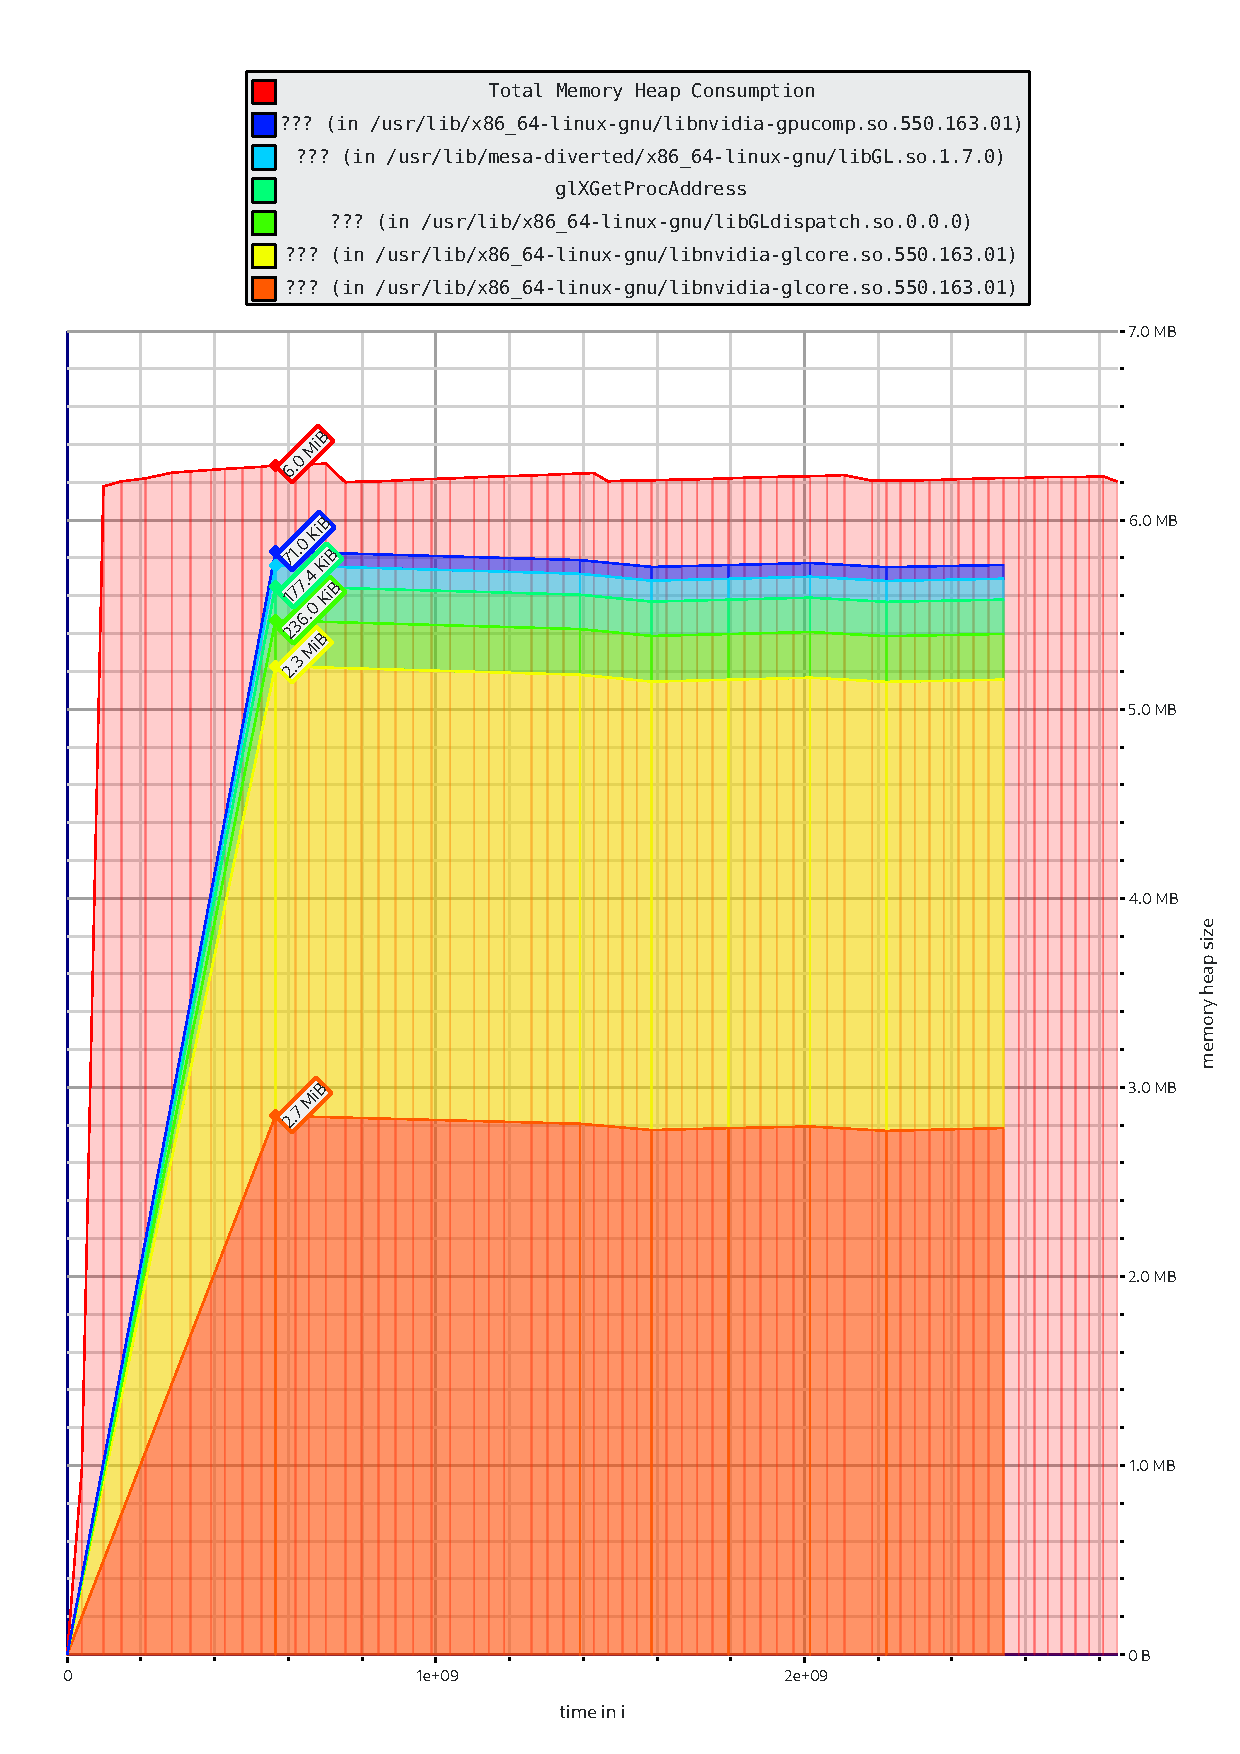
\includegraphics[width=1.0\textwidth]{figures/graphs/massif-visualizer-polygon.pdf}
    \caption{Gráfica que representa el uso de memoria en la prueba del polígono}
    \label{fig:massif-visualizer-polygon}
\end{figure}

\begin{figure}[htp]
    \centering
    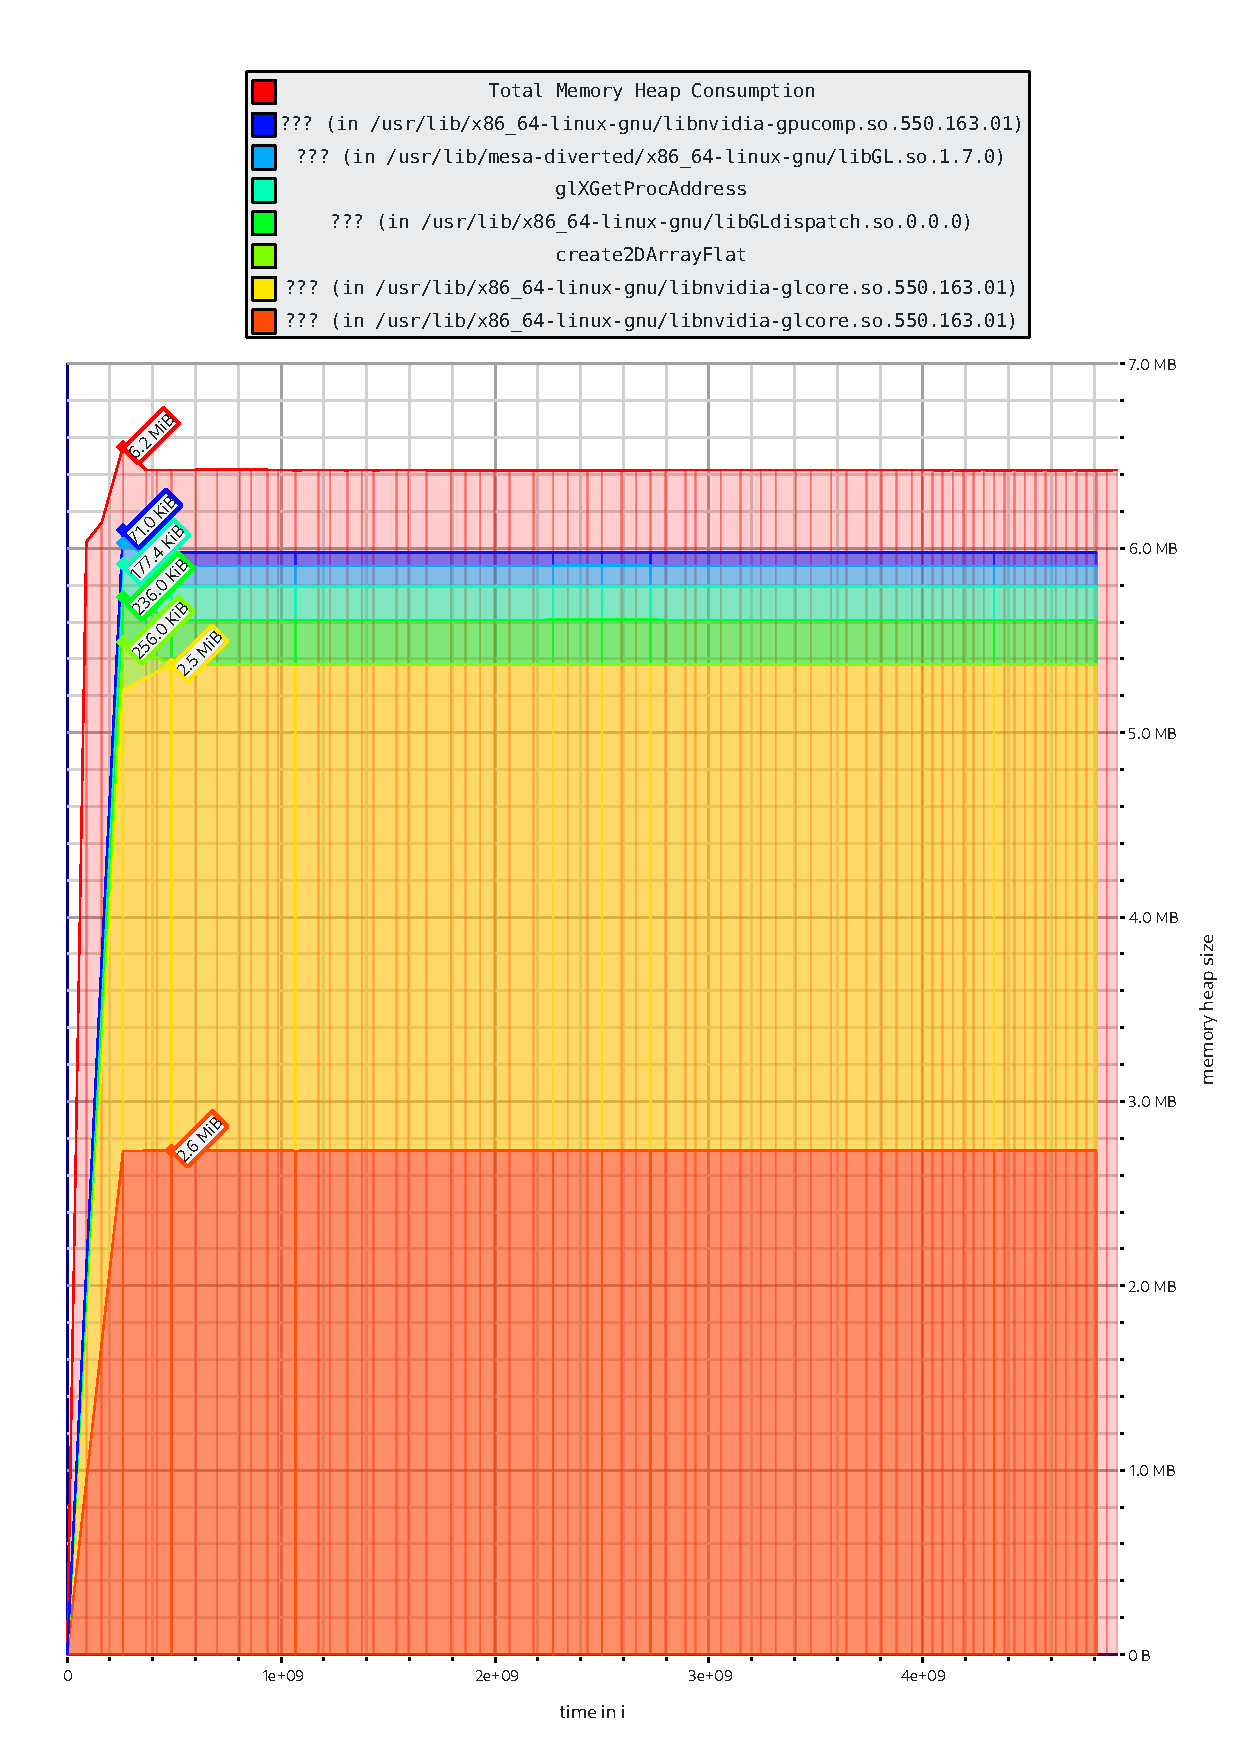
\includegraphics[width=1.0\textwidth]{figures/graphs/massif-visualizer-animation.pdf}
    \caption{Gráfica que representa el uso de memoria en la prueba de animación}
    \label{fig:massif-visualizer-animation}
\end{figure}

\section{Análisis de CPU} \label{sec:cpu-analysis}

\begin{table}[htp]
\centering

    % Esta primera línea define las columnas de la tabla. Los posibles tipos de columna son:
    % c: texto centrado
    % l: texto alineado a la izquierda
    % r: texto centrado a la derecha
    % p: columna de ancho fijo
    % Las columnas tienen ancho dinámico según la anchura máxima de los elementos que contengan.

    % Las columnas l/r/c no parten el texto en filas diferentes si éste es demasiado largo. Para ello, puede utilizar el tipo de columna de ancho fijo "p".
    
    % Las barras verticales | se usan para definir los bordes verticales de la tabla. Pruebe a eliminar algunas y observe qué ocurre.
    \begin{center}
    \begin{tabular}{ | l | l | l | }
        
        % A continuación van las filas de la tabla. En cada fila, las columnas se separan con el carácter &
        % Para terminar una fila se usa \\
        % Para incluir un borde horizontal entre filas se usa \hline
        
        % Cabecera con textos en negrita:
        \hline
        \textbf{Measure} & \textbf{Animation}  & \textbf{Polygon} \\
        \hline
        \textbf{Task clock (miliseconds)}  & 3,561 & 3,574 \\
        \hline
        \textbf{CPUs utilized}  & 0.367 & 0.915 \\
        \hline
        \textbf{Page faults} & 3,609  & 3,554\\
        \hline
        \textbf{Frequency (GHz)} & 3.187 & 3.268 \\
        \hline
        \textbf{Instructions per cycle} & 1.04 & 0.77 \\
        \hline
        \textbf{Branches per second} & 665.660 & 550.479 \\
        \hline
        \textbf{Branch misses percentage} & 1.21 & 1.14 \\
        \hline
        \textbf{Time elapsed (seconds)} & 9.7086 & 3.9050 \\
        \hline
        \textbf{Time user (seconds)} & 2.2427 & 1.1099 \\
        \hline
        \textbf{Time system (seconds)} & 1.3618 & 2.4674 \\
        \hline
        \textbf{Context switches} & 18,666 & 1,914 \\
        \hline
        \textbf{CPU migrations} & 331 & 26 \\
        \hline
        
    \end{tabular} 
    \end{center}
    
    \caption{Comparación de los resultados de la herramienta \textit{perf} durante la ejecución de las pruebas.}
    
    \label{tbl:perf-comparison}
\end{table}

Utilizando la herramienta \textit{perf}, con la subherramienta \textit{stat} \cite{webPerfStat}, se han recopilado datos del rendimiento de la \textit{CPU} durante la ejecución de las pruebas y se han presentado en la tabla \ref{tbl:perf-comparison}, donde para las pruebas de \textbf{animación} y \textbf{polígono} se toman diferentes \textbf{medidas}.

\begin{itemize}
    \item El tiempo tomado por ambas tareas es similar, aunque para la animación se haya utilizado un tercio de la cantidad de \textit{CPUs} que en polígono; lógico, ya que en la prueba de animación se divide la carga entre \textit{GPU} y \textit{CPU} más que en la prueba del polígono: el sistema de animaciones y algunas operaciones matriciales son tarea de la \textit{CPU}, mientras que la \textit{GPU} maneja operaciones de memoria y matriciales y renderizado.
    
    \item La frecuencia de la \textit{CPU} utilizada en las pruebas es \textit{3.5 GHz}, lo que concuerda con los resultados obtenidos.
    
    \item El \textit{IPC} o instrucciones por ciclo son mayores en la prueba de animación.
    
    \item Las migraciones de \textit{CPU} se relacionan con un traslado del proceso entre núcleos, semejante a los cambios de contexto, aunque este último se relaciona con el comportamiento del \textit{scheduler} o \textbf{planificador} del sistema operativo; ambos valores son más altos en la prueba de animación, debido a mayor número de bibliotecas involucradas y la necesidad de realizar múltiples tareas al mismo tiempo.

    \item El porcentaje de saltos fallidos es muy bajo, lo que indica una correcta predicción en la ejecución.

    \item La duración en segundos del usuario junto al sistema sí concuerda en la prueba del polígono, aunque no en la animación, ya que esta última no finaliza en cuanto se completa la renderización de los fotogramas.
    
\end{itemize}

\section{Conclusiones}
En este capítulo se han diseñado pruebas sobre los programas creados, midiendo el rendimiento y analizando los resultados. Se ha observado que, según el escenario, puede sufrir más el rendimiento de la \textit{CPU} o la \textit{GPU}: en la prueba de polígonos, era peor el rendimiento de la \textit{CPU}, y en la de animaciones, era peor el rendimiento de la gráfica.
    \chapter{Conclusiones}\label{cap:conclusiones}

En este proyecto se han desarrollado bibliotecas para el uso de \textit{OpenGL}: bibliotecas de configuración, creación de geometría, animaciones, funciones auxiliares de \textit{C} y gestión de errores. Todas estas bibliotecas se han utilizado en programas: a destacar, el programa de animación, que realiza una serie de transformaciones programables a un polígono regular y se renderiza en pantalla. 

Para exprimir y medir las funcionalidades aquí desarrolladas, se han realizado pruebas en las que todas ellas se ven involucradas. Luego, con \textit{R} y \textit{gnuplot}, se toman cómputos numéricos sobre los datos recogidos y gráficas para visualizarlos con detalle.

\section{Líneas futuras}

Este proyecto sólo es una base para los muchos caminos por los que podría expandirse. A continuación, se enunciarán las posibles líneas futuras que se han contemplado: mejoras de rendimiento, nuevas características, integraciones con otros programas y comparativas.

\begin{itemize}

    \item Mejorar el sistema de animación para permitir geometría tridimensional.

    \item Capacidad de importación de modelos. Se examinó la posibilidad de incorporar \textit{Assimp} con el fin de probar geometría más compleja y diferente.

    \item Algoritmos de triangulación, para transformar geometría compleja en triángulos simples, amigables con la \textit{GPU} y más sencillos de procesar.

    \item Integración con otros programas como extensión y observar ventajas y desventajas. Como caso concreto, \textit{Godot} ofrece una tecnología para interactuar con código \textit{C/C++} llamado \textit{GDExtension} \cite{webGodotGDExtension}, aún en estado experimental; en el caso de ser insuficiente, pueden usarse los módulos personalizados de \textit{C/C++} que también ofrece \textit{Godot} \cite{webGodotCModules}.

    \item Crear comparativas de los tiempos de ejecución respecto a otros programas, como el ya mencionado previamente \textit{Godot}.

    \item Mejora al sistema de animación, permitiendo fácilmente crear caminos distintos para diferentes geometrías y cargar la animación desde un fichero.

    \item Mejora a la biblioteca de \textit{shaders}, abstrayendo aún más las funciones principales, como \textit{initAnimationData}, \textit{initGLData} y \textit{initGLShaders}, incluso permitiendo crear \textit{shaders} básicos sin programar \textit{GLSL}.

\end{itemize}

    \chapter{Anexos} \label{chp:Annex}

A continuación, se incluyen el repositorio de Gitlab utilizado durante el proyecto \url{https://gitlab.com/ivabarlay/renderergl2d} \ref{fig:qr-code}.

\begin{figure}[htp]
    \centering
    
\includegraphics[width=0.6\textwidth]{figures/qr_code.png}
    \caption{QR del repositorio de código}
    \label{fig:qr-code}

\end{figure}


    % Bibliografía
    \bibliographystyle{unsrtnat}
    \bibliography{bibliografia.bib}
        

% Fin del documento
\end{document}
